\documentclass[a4paper,11pt]{article}

\usepackage[T1]{fontenc}
\usepackage{xltxtra}
\usepackage[francais]{babel}
\usepackage{fancyhdr}

\usepackage{epsfig}
\usepackage{calc}
\usepackage{url}
\usepackage{boxedminipage}

\usepackage{titlesec}
%Pour enlever cette merde de chapter!
%\titleformat{\chapter}[hang]{\bf\huge}{\thechapter}{2pc}{}
\usepackage{graphicx}
%\usepackage{svg}
\usepackage{xcolor}
\usepackage{float}

\usepackage{tabularx}
\usepackage[colorlinks=true, linkcolor=black, citecolor=violet, urlcolor=blue]{hyperref}
\usepackage[sort, authoryear]{natbib}
\usepackage{subcaption}
\bibpunct{[}{]}{,}{n}{,}{,}

\usepackage{amsmath}
\usepackage{amssymb}
\usepackage{listings}
\usepackage[toc]{appendix}
\renewcommand{\appendixtocname}{Annexes}
% --------------------------------
%Pour compiler sur Manjaro        
\usepackage[utf8]{inputenc}
\usepackage{algorithmicx}
\usepackage{algpseudocode}
%% \usepackage[latin1]{inputenc}
% --------------------------------
%Pour les tableaux multi-colonnes
\usepackage{multirow}
\usepackage{tocloft}
\setcounter{page}{1}
\pagenumbering{Roman}
%%\onehalfspacing

\renewcommand{\lstlistingname}{Algorithme}
\renewcommand{\lstlistlistingname}{Liste des algorithmes}

\renewcommand{\cftdotsep}{\cftnodots}
%%%%%%%%%%%%%%%%%%%%%%%%%%%%%%%%%%%%%%%%%%%%%%%%%%%%%%%%%%%
%%%%%%%%%%%%%%%%%%%%%%%%%%%%%%%%%%%%%%%%%%%%%%%%%%%%%%%%%%%
%% Définitions à personnaliser 

%% Pour les noms, utilisez la première lettre du prénom suivi du 
%% nom de famille (première lettre majuscule, reste en minuscule).


%%%% Indiquer le nom de l'encadrant ci-dessous:

\def\nomEncad{Martin \textsc{Quinson}}

%% Si le projet est co-encadré indiquer les deux noms à la suite dans 
%% Le même champs


%%%% Indiquer les noms des étudiants participant ci-dessous:

\def\nomEtudA{Louisa \textsc{Bessad}}

%% Si le projet est encadré par moins de 4 étudiants laissez
%% les variables inutiles vides


%%%% Indiquer la référence (numero) et le nom du sujet ci-dessous:

\def\refProjet{Numéro Projet} 
\def\titreProjetCourt{Titre court}
\def\titreProjetLong{Real-time online emulation of real applications on SimGrid with Simterpose}

%% Le titre court ne doit pas faire plus d'une vingtaine de caractère
%% résumez le à quelques mots essenciels


%%%% Indiquer le type de document et sa version ci-dessous:

\def\typeDoc{Rapport final}
 
%% - Rapport intermédaire
%% - Rapport final

%\let\origsec\section
%\renewcommand{\section}[1]{\newpage\origsec{#1}}



%%%%%%%%%%%%%%%%%%%%%%%%%%%%%%%%%%%%%%%%%%%%%%%%%%%%%%%%%%%
%%%%%%%%%%%%%%%%%%%%%%%%%%%%%%%%%%%%%%%%%%%%%%%%%%%%%%%%%%%
%% Définitions à ne pas modifier
 
%%%% ||| Mise en page verticale ||| 
\setlength{\voffset}{-1in} % a4:reste 297mm pour les 5 suivants:
\setlength{\topmargin}{15mm}         % avant l'en-tête
\setlength{\headheight}{20mm}        % hauteur de l'en-tête 
\setlength{\headsep}{10mm}            % entre l'en-tête et le corps
\setlength{\textheight}{220mm}       % hauteur du corps
\setlength{\footskip}{12mm}          % pied de page par rapport au corps 
%\setlength{\footlength}{2em}

%%%%% --- Mise en page horizontale ---
\setlength{\hoffset}{-1in} % a4:reste 210mm 
\setlength{\oddsidemargin}{25mm}     % entre hoffset et le corps
\setlength{\evensidemargin}{25mm}    % entre hoffset et le corps
\setlength{\marginparwidth}{0mm}     % largeur de la marge
\setlength{\marginparsep}{0mm}       % séparateur corps marge
\setlength{\textwidth}{160mm}        % largeur du corps

%\usepackage{fullpage}
%\setlength{\headheight}{20mm}        % hauteur de l'en-tête 
%\setlength{\headsep}{10mm}            % entre l'en-tête et le corps
%\setlength{\textheight}{200mm}
%\setlength{\footskip}{0mm}          % pied de page par rapport au corps 

\def\annee{2015}



%%%%%%%%%%%%%%%%%%%%%%%%%%%%%%%%%%%%%%%%%%%%%%%%%%%%%%%%%%%
%% Début du document

\begin{document}
\begin{titlepage}

\newcommand{\HRule}{\rule{\linewidth}{0.5mm}} % Defines a new command for the horizontal lines, change thickness here

\center % Center everything on the page
 
%----------------------------------------------------------------------------------------
%	HEADING SECTIONS
%----------------------------------------------------------------------------------------

\textsc{\LARGE Université Pierre et MArie Curie}\\[0.44cm] % Name of your university/college
\textsc{\Large Master informatique}\\[0.44cm] % Major heading such as course name
\textsc{\large Systèmes et Applications Répartis}\\[1.44cm] % Minor heading such as course title

\textsc{\LARGE Loria}\\[0.44cm] % Name of your university/college
\textsc{\Large Équipe VERIDIS}\\[1.44cm] % Major heading such as course name

%----------------------------------------------------------------------------------------
%	TITLE SECTION
%----------------------------------------------------------------------------------------

\HRule \\[0.4cm]
{ \huge \bfseries Real-time online emulation of real applications on SimGrid with Simterpose}\\[0.4cm] % Title of your document
\HRule \\[1.44cm]
 
%----------------------------------------------------------------------------------------
%	AUTHOR SECTION
%----------------------------------------------------------------------------------------

\begin{minipage}{0.4\textwidth}
\begin{flushleft} \large
\emph{Étudiante:}\\
Louisa \textsc{Bessad} % Your name
\end{flushleft}
\end{minipage}
~
\begin{minipage}{0.4\textwidth}
\begin{flushright} \large
\emph{Encadrant} \\
Martin \textsc{Quinson} % Supervisor's Name
\\\vspace{1.44cm} \emph{Rapporteur:} \\ Sébastien
\textsc{Monnet}
\end{flushright}
\end{minipage}\\[1.5cm]

% If you don't want a supervisor, uncomment the two lines below and remove the section above
%\Large \emph{Author:}\\
%John \textsc{Smith}\\[3cm] % Your name

%----------------------------------------------------------------------------------------
%	DATE SECTION
%----------------------------------------------------------------------------------------

{\large \today}\\[1.5cm] % Date, change the \today to a set date if you want to be precise

%----------------------------------------------------------------------------------------
%	LOGO SECTION
%----------------------------------------------------------------------------------------

%\includegraphics{Logo}\\[1cm] % Include a department/university logo - this will require the graphicx package

\includegraphics[scale=0.2]{Pictures/png/UPMC_sorbonne.png}\hspace{3cm}

\includegraphics[scale=0.1]{Pictures/loria_logo.jpg}

%----------------------------------------------------------------------------------------

\vfill % Fill the rest of the page with whitespace
\end{titlepage}
\clearpage
%\vfill

\newpage
\thispagestyle{empty}
\mbox{}
\newpage
\setcounter{page}{1}
\tableofcontents
%\vfill
\newpage
%% \mbox{}
%% \newpage

\listoffigures
\newpage

\listoftables
\newpage

\lstlistoflistings
\newpage
\thispagestyle{empty}
\mbox{}
\newpage

%Abstract
%\begin{abstract}
 %TODO
  %% Dans le cadre de ce stage nous allons nous intéresser aux applications ditribuées à large échelle et comment on peut les tester et évaluer leurs performances via une combinaison d'émulation et de simulation en utilisant SIMGRID et Simterpose qui sont deux projets européens. SIMGRID a été lancé en 1999 pour étudier des algorithmes d'ordonnancement sur des plateformes hétérogènes dans un environnement distribué et faciliter leur programmation. Il fournit les outils de base nécessaire à la simulation de ce type d'applications. Simterpose s'insère dans le projet SIMGRID afin de pouvoir étudier des applications complètes et pas uniquement leur modèle que l'on fournit habituellement en paramètre au simulateur. Le but est de faire de l'émulation en utilisant un simulateur que sera SIMGRID. Puisque nous nous intéressons aux applications distribuées notre émulateur doit pouvoir\textit{i)} exécuter un grand nombre d'instances d'une même application sur un même système afin de pouvoir debugguer, \textit{ii)} évaluer des applications ayant de nombreuses condition d'exécution (simple n\oe ud, réseau complet), \textit{iii)} collecter les informations concernant l'application pendant qu'elle s'exécute.
%\end{abstract}
%\newpage

%%%%%%%%%%%%%%%%%%%%%%%%%%%%%%%%%%%%%%%%%%%%%%%%%%%%%%%%%%%
%% Définition des en-têtes et pied de pages
\pagestyle{fancyplain}
%\fancyhead{}
%\fancyfoot{}
%
\fancyhead[L]{\textsc{Université Pierre et Marie Curie} \\ {\color{white} b} \\ \nomEtudA}
\fancyhead[C]{\textbf{Rapport final}}%\\\titreProjetCourt}}
\fancyhead[R]{\textsc{LORIA} \\ {\color{white} b} \\ \nomEncad}

\fancyfoot[L]{
\includegraphics[width=3cm]{Pictures/png/UPMC_sorbonne.png}}
\fancyfoot[C]{\textbf{\thepage}}
\fancyfoot[R]{
\includegraphics[width=4cm]{Pictures/loria_logo.jpg}}

%\lhead[\fancyplain{}{\texttt{Université Pierre et Marie Curie}\\
%          Master Informatique\\ UE \textbf{PSAR} fév. \annee \\ \nomEncad}]
%      {\fancyplain{}{\textsc{Université Pierre et Marie Curie}\\
%          Master Informatique\\ UE \textbf{PSAR} \annee \\ \nomEncad}}
%\chead[\fancyplain{}{\textbf{Projet \refProjet\\\titreProjetCourt}}]
%      {\fancyplain{}{\textbf{Projet \refProjet\\\titreProjetCourt}}}
%\rhead[\fancyplain{}{\nomEtudA\\\nomEtudB}]
%      {\fancyplain{}{\nomEtudA\\\nomEtudB}}
%\lfoot[\fancyplain{}{\epsfig{figure=UPMC_sorbonne.eps,width=3cm}}]
%      {\fancyplain{}{\epsfig{figure=UPMC_sorbonne.eps,width=3cm}}}
%\cfoot[\fancyplain{}{\textbf{\thepage/\pageref{fin}}}]
%      {\fancyplain{}{\textbf{\thepage/\pageref{fin}}}}
%\rfoot[\fancyplain{}{\typeDoc}]
%      {\fancyplain{}{\typeDoc}}


%%%%%%%%%%%%%%%%%%%%%%%%%%%%%%%%%%%%%%%%%%%%%%%%%%%%%%%%%%%



{\color{white} blabla} \vspace{7cm}

Ce stage se déroule au Loria, Laboratoire Lorrain de Recherche en Informatique
et ses Applications, unité mixte de recherche commune à plusieurs
établissements: le CNRS, l'INRIA, et l' Université de Lorraine. Le LORIA a pour
mission la recherche fondamentale et appliquée en sciences informatiques et ce,
depuis sa création, en 1997.

L'encadrement est assuré par Martin Quinson au sein de l'équipe VERIDIS, dont les sujets de recherches sont la conception de méthodes pour les systèmes distribués et d'outils pour la vérification et la validation de systèmes.



\newpage

{\color{white} blabla} \vspace{7cm}


Je voudrais remercier mon tuteur Martin Quinson pour m'avoir permis d'effectuer ce stage, durant lequel j'ai beaucoup appris.

Je tiens également à remercier mon encadrant universitaire Sébastien Monnet pour ses précieux conseils.

\newpage

\setcounter{page}{1}
\pagenumbering{arabic}
% Content

\section{Introduction}

%% intro/objectif: virtualisation légère d'applications distribuées (tester des applications distribuées réelles: test regression et performance, légère car on veut tester des centaines d'instances)

%% Applications: stockage distribué (CEPH, TAHOE/LAFS) et RT event processing (Storm)

Dans le cadre de ce stage, nous allons nous intéresser aux applications
distribuées. Il s'agit d'applications dont une partie ou la totalité des
ressources n'est pas localisée sur la machine où l'application s'exécute, mais
sur plusieurs machines distinctes. Ces dernières communiquent entre elles via le
réseau pour s'échanger les données nécessaires à l'exécution de
l'application. Les applications distribuées ont de nombreux avantages: elles
permettent notamment d'augmenter la disponibilités des données en se les
échangeant, comme les applications Torrent (BitTorrent, $µ$Torrent...). Grâce au
projet BOINC\footnote{\url{https://boinc.berkeley.edu/}} par exemple, on peut
partager la puissance de calcul inutilisée de sa machine. Depuis une dizaine
d'années, la popularité de ces applications distribuées ne cesse de croître. On
peut notamment penser aux applications de stockage de données
LAFS\footnote{\url{https://tahoe-lafs.org/trac/tahoe-lafs}} et
CEPH\footnote{\url{http://ceph.com/}}. La première apporte un stockage robuste
qui préserve les données même si un site est physiquement détruit. La seconde
souhaite fournir performance, fiabilité et scalabilité.  Elles deviennent de
plus en plus complexes avec des contraintes et des exigences de plus en plus
fortes, en particulier au niveau des performances et de l'hétérogénéité des
plateformes et des ressources utilisées. Il est donc de plus en plus
difficile de créer de telles applications (absence d'horloge et mémoire
centrale, deadlock, race, famine) mais aussi de les tester.  En effet, malgré
l'évolution des applications distribuées, les protocoles d'évaluation de leurs
performances n'ont que peu évolués.
\newline

Actuellement, il existe trois façons principales de tester le comportement
d'applications distribuées \citep{gustedt2009experimental}: l'exécution sur
plate-forme réelle, la simulation et l'émulation.

La première solution consiste à exécuter réellement l'application sur un parc de
machines et d'étudier son comportement en conditions réelles. Cela permet de la
tester sur un grand nombre d'environnements. L'outil créé et développé en partie
en France pour cela est \textbf{Grid'5000}\footnote{Infrastructure de 8000 c\oe
  urs répartis dans la France entière crée en
  2005. \\ \url{https://www.grid5000.fr/mediawiki/index.php/Grid5000:Home}}\citep{GRID5000},
un autre outil développé à l'échelle mondiale est
\textbf{PlanetLab} \footnote{Crée en 2002, cette infrastructure de test compte
  aujourd'hui 1340 c\oe urs. \\ \url{http://www.planet-lab.org}}. Néanmoins,
pour mettre en \oe uvre ces solutions complexes, il faut disposer des
infrastructures nécessaires pour effectuer les tests. Il faut également écrire
une application complète capable de gérer toutes ces ressources
disponibles. Enfin, du fait du partage des différentes plateformes entre
plusieurs utilisateurs, les expériences sont difficilement reproductibles.

La seconde solution consiste à faire de la simulation: on modélise ce que l'on
souhaite étudier (application et/ou environnement) via un programme appelé
simulateur. Dans ce cas, pour pouvoir tester des applications distribuées sur un
simulateur, on doit d'abord abstraire l'application ainsi que l'environnement
d'exécution. Pour cela, on identifie les propriétés de l'application et de son
environnement puis on les transforme à l'aide de modèles mathématiques. Ainsi,
on va exécuter dans le simulateur le modèle de l'application et non
l'application réelle, dans un environnement également modélisé. Cette solution
est donc facilement reproductible, plus simple à mette en \oe uvre, et permet de
prédire l'évolution du système étudié grâce à l'utilisation de modèles
mathématiques. De nos jours, les simulateurs tel que
\textbf{SimGrid}\citep{CASANOVA:SimGrid, MARTIN:SimGrid} peuvent simuler des
applications distribuées mettant à contribution des milliers de
n\oe uds. Néanmoins, avec la simulation on ne peut valider qu'un modèle et non
l'application elle-même.

La troisième solution consiste à faire de l'émulation: on exécute réellement
l'application mais dans un environnement virtualisé grâce à un logiciel,
l'émulateur. Ce dernier joue le rôle d'intercepteur pour virtualiser
l'environnement d'exécution.
%On fera ainsi croire à l'application qu'elle s'exécute sur une machine autre que l'hôte.
Cette solution représente un intermédiaire entre la simulation et l'exécution
sur plateforme réelle visant à résoudre les limitations de ces deux
solutions. En effet, les actions de l'application sont réellement exécutées sur
la machine hôte (la machine réelle sur laquelle s'exécute l'émulation) et grâce
à la virtualisation, l'application pense être dans un environnement différent de
la machine réelle. De plus, cela évite d'avoir deux versions de l'application en
terme de code: une pour la simulation et une pour la production. L'émulation
peut-être faite \textit{off-line} (on sauvegarde les actions de l'application
sur disque et on les rejoue plus tard dans un simulateur) ou \textit{on-line}
(on bloque l'application le temps que le temps de réponse de la plateforme
virtualisée soit calculé).

%% Il existe deux types d'émulation pour les applications distribuées; la
%% virtualisation standard et la légère. On parle de virtualisation légère quand on
%% souhaite tester des applications sur une centaine d'instances.

Au cours de ce stage, nous allons nous intéresser plus particulièrement à l'exécution d'applications distribuées arbitraires au dessus de la plateforme de simulation SimGrid. Pour cela, nous allons présenter en section \ref{section:emulation} les méthodes utilisées
pour faire de la virtualisation %% légère: limitation et interception
. Puis en
section \ref{section:sota} nous présenterons les projets permettant de faire de
l'émulation pour tester des applications dans un environnement
distribué. Ensuite, nous expliquerons en section \ref{section:simterpose},
pourquoi dans le cadre du projet Simterpose c'est la virtualisation légère par
interception qui a été choisie et comment elle fonctionne. Pour finir, nous
concluerons en section \ref{section:ccl}.

\newpage
\section{Pourquoi choisir l'émulation simulée}

Il existe trois façons de tester des applications distribuées. La première consiste à exécuter réellement l'application sur un parc de machines et d'étudier le comportement de l'application en temps-réel, ce que fait actuellement \textbf{Grid'5000} {\color{red}mettre citation}. Néanmoins pour mettre en \oe uvre cette solution complexe il faut disposer des architectures nécessaires pour effectuer les tests. De part le partage des différentes plateformes entre divers utilisateurs les expériences ne sont pas forcément reproductibles. Une deuxième solution consiste à simuler l'exécution des applications à l'aide d'un simulateur tel que \textbf{SIMGRID} {\color{red}mettre citation}. On doit alors modéliser l'application ainsi que l'environnements d'exécution grâce à des modèles mathématiques. Le problème avec la simulation est que l'on exécute pas vraiment l'application, on ne peut alors valider qu'un modèle et pas l'application puisqu'on réécrit l'application selon le modèle. Un des buts du projet étant de tester les applicationis sans avoir accès à leur code source, on ne peut donc pas choisir cette solution ou pas toute seule en tout cas. La troisième solution consiste à faire de l'émulation, c'est-à-dire que nous allons exécuter réellement l'applications mais dans en environnement virtuels. Ainsi nous aurons un simulateurs qui gérera l'environnement, l'application qui s'exécutera réellement sur la machine hôte et une API qui fera le lien entre l'application qui s'exécute et l'environnement simulé. On fera ainsi croire à l'application qu'elle s'exécute sur une machine autre que l'hôte. Il existe deux façons de faire de l'émulation: la dégradation et l'interception. Dans la première on rajoute la couche d'émulation au-dessus de la plateforme réelle (comme un hyperviseur pour une VM). Mais cela nous empêche d'émuler des machines plus puissante que l'hôte car le délai de réponse géré par l'émulateur ne peut-être inférieur à celui de l'hôte sinon l'hôte n'a pas le temps de faire les calculs nécessaires à l'application. Cette solution choisie par \textbf{Distem}{\color{red}mettre citation} est donc limitée à la capacité des plateformes à notre disposition. Dans le cas de l'interception pour faire croire à l'application qu'elle s'exécute sur une machine autre que l'hôte on va attraper toutes ses communications via une API du simulateur qui ensuite les transmetra au simulateur. Ce dernier s'occupera de calculer le temps de réponses de ces commumnications en se basant sur les performances de la machine qu'on est en train de simuler. Les calculs seront effectués sur la machine hôte mais le temps de réponse à l'application sera géré par le simulateur en fonction de l'architecture que l'on simule en utilisant le temps d'exécution de la machine hôte injectés dans le simulateur et en comparant les performances des deux architectures. Ainsi le temps de l'application sera celui du simulateur et non le temps réel. Cette solution est implémentée dans \textbf{Simterpose}{\color{red}mettre citation}. Dans notre cas d'émulation simulation, nous allons utiliser SIMGRID comme simulateur et Simterpose comme API de ce simulateur. Nous aurons donc Simterpose qui permettra d'utiliser SIMGRID avec des applications réelles en leur faisant croire qu'elles s'exécutent sur des machines distribuées. Maintenant que nous savons comment nous allons tester les applications distribuées nous allons voir comment fonctionne notre ``émulateur'' Simterpose.

\subsection{Virtualisation standard}
\label{section:limitation}
%% \begin{itemize}
%% \item principe: limiter l'accès aux ressources par exemple (cgroup, netstat, cpuburner), temps d'un SEB (bench avec netlink, limiter (cap))
%% \item avantage plus simple
%% \item désavantages: host>>target, modèle à vérifier, contrôle expérimental fin
%% \end{itemize}

Avec cette première méthode, illustrée Fig.\ref{TYPE_VIRTUALISATION}, on place la couche d'émulation au-dessus de la
plateforme réelle (comme un hyperviseur pour une VM). De fait, la puissance de
l'émulateur dépend de la puissance de la machine hôte et ne peux donc pas
dépasser les capacités de cette dernière. De plus, en choisissant de placer
l'émulation comme une surcouche, cela permet de limiter l'accès aux ressources
pour les applications. En effet, elles ne pourront pas passer la couche
d'émulation pour accéder aux ressources localisées sur la machine hôte. Les
requêtes des applications distribuées seront arrêtées par l'émulateur. C'est lui
qui s'occupera de récupérer les ressources demandées par les applications. Il
existe différents outils permettant de mettre en place cette virtualisation, on
trouve notamment \textbf{cgroups} \citep{cgroups} et \textbf{cpuburner} \citep{canon2006wrekavoc, buchert2011methods} pour le système et \textbf{iptables} \citep{netfilter_iptables, iptables_man} pour le réseau. L'émulation par limitation a l'avantage d'être simple à mettre en \oe uvre puisque
l'on se base sur la machine hôte. Néanmoins elle est assez contraignante du fait
qu'on ne puisse pas émuler des architectures plus performantes que l'hôte.

\subsection{Emulation par interception}
\label{section:interception}
%% principe: interception des actions et médiation (pas juste interception et rejeu). Intercepter des symboles pour en changer l'effet

Dans le cas de l'émulation par interception, illustrée
Figure \ref{Virtu_interception} , pour mettre en place un environnement distribué
émulé sur lequel les applications penseront s'exécuter, deux outils vont être
utilisés; un simulateur pour virtualiser l'environnement d'exécution, et un
émulateur qui va attraper toutes les communications de l'application avec l'hôte
et qui les transmettra ensuite au simulateur.

 \begin{figure}[H]
   \centering 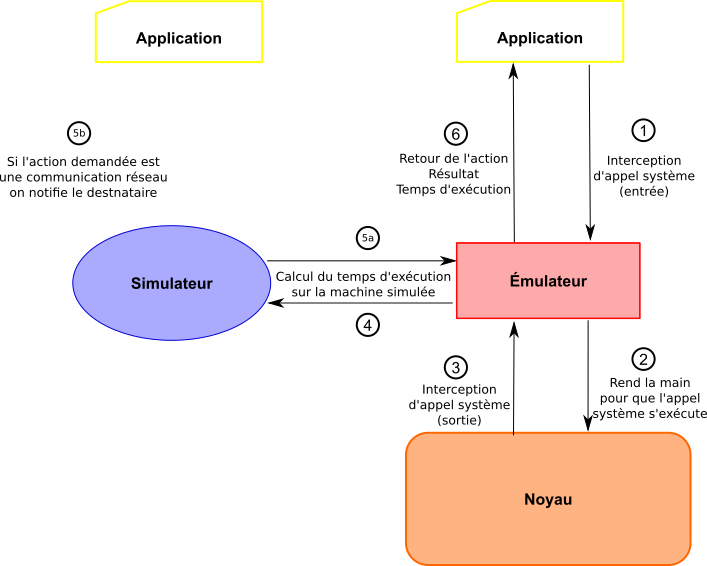
\includegraphics[scale=0.5]{Pictures/png/Emulation_fonctionnement}
   \caption{Fonctionnement de l'émulation par interception.}
   \label{INTERCEPTION}
 \end{figure}
 
 Une application distribuée peut vouloir interagir avec son environnement soit
 pour effectuer de simples calculs, soit pour effectuer des communications avec
 d'autres applications sur le réseau. Quand l'émulateur intercepte une
 communication venant d'un des processus d'une application, il modifie les
 caractéristiques de la communication pour qu'elle puisse s'exécuter sur la
 machine hôte. Il fait la même chose lorsque cette dernière envoie une réponse à
 l'application. En parallèle, l'émulateur demande au simulateur de calculer le
 temps d'exécution de l'action dans l'environnement virtuel pour l'action
 demandée par l'application. L'émulateur envoie ce temps à l'application en plus
 du résultat du calcul demandé pour mettre à jour son horloge. Ainsi, les
 calculs sont réellement exécutés sur la machine, les communications réellement
 émises sur le réseau géré par le simulateur et c'est le temps de réponse qu'il
 fourni qui va influencer l'horloge de l'application. Finalement, les
 applications ne communiquent plus directement entre elles.

 
Pour intercepter ces actions, il faut d'abord choisir à quel niveau se placer.
En effet, une application peut communiquer avec le noyau via différentes
abstractions, Figure \ref{AS_Communication}. Elle peut soit utiliser les
fonctions d'interaction directe avec le noyau que sont les appels systèmes, soit
utiliser les différentes abstractions fournies par le système d'exploitation:
bibliothèques (fonctions de la libc par exemple) ou les fonctions POSIX dans le
cas d'un système UNIX.

Nous allons donc voir comment on peut intercepter et modifier des actions au
niveau de l'application (fichier source puis binaire), des appels système et
des appels de fonctions. Par la suite nous appelerons médiation l'ensemble des
modifications effectuées par l'émulateur sur les actions interceptées.

\begin{figure}[H]
 \centering
 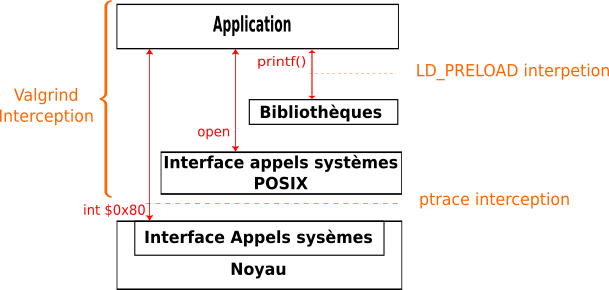
\includegraphics[scale=0.75]{Pictures/png/Communication_application_noyau_v3.png}
 \caption{Communications possibles entre le noyau et une application.}
 \label{AS_Communication}
\end{figure}

Dans cette section, nous avons pu voir qu'il existe différents types de virtualisation. Puisque nous souhaitons pouvoir utiliser des milliers de plateformes durant nos exécutions nous ne pouvons utiliser la virtualisation complète de la machine. La virtualisation légère par dégradation est également exclue car nous devons pouvoir émuler des machines plus performantes que l'hôte. La virtualisation légère par interception semble être celle qui correspond le mieux aux besoins de notre projet. Pour pouvoir être mise en place elle nécessite d'utiliser des outils d'interception pour les différentes actions de l'application. Il existe différents outils permettant de faire cela, nous allons les présenter dans la section suivante.


\newpage
\section{Outils pour la virtualisation légère}
\label{section:tools}

Afin d'intercepter les actions d'une application il faut d'abord choisir à quel
niveau se placer.  En effet, une application peut communiquer avec le noyau via
différentes abstractions, Figure \ref{AS_Communication}. Elle peut soit utiliser
les fonctions d'interaction directe avec le noyau que sont les appels systèmes,
soit utiliser les différentes abstractions fournies par le système
d'exploitation: bibliothèques (fonctions de la \texttt{libc} par exemple) ou les
fonctions POSIX dans le cas d'un système UNIX.

Nous allons donc voir comment on peut intercepter et modifier des actions au
niveau de l'application (fichier source puis binaire), des appels système et
des appels de fonctions. Par la suite nous appelerons médiation l'ensemble des
modifications effectuées par l'émulateur sur les actions interceptées.

\begin{figure}[H]
 \centering
 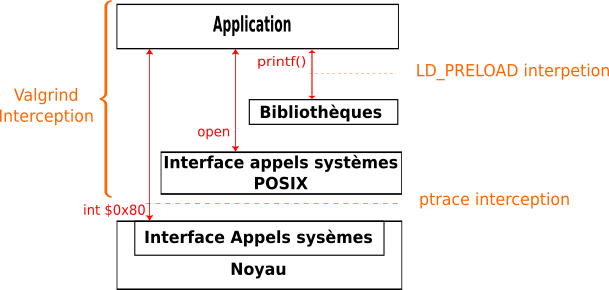
\includegraphics[scale=0.75]{Pictures/png/Communication_application_noyau_v3.png}
 \caption{Communications possibles entre le noyau et une application.}
 \label{AS_Communication}
\end{figure}

\subsection{Action sur le fichier source}
\label{subsection:source}
%% reimplem SMPI (trop spé) ,source to source/ pass LLVM( gcc+libc=consanguin) 
%% , Coccinelle
Le premier niveau auquel on peut se placer pour intercepter les actions est le fichier source de l'application. On peut réécrire les parties qui nous intéressent avant de compiler le code.

Un premier outil pour cela est le programme Coccinelle\footnote{Coccinelle project \url{http://coccinelle.lip6.fr/}}. Il permet de trouver et transformer automatiquement des parties spécifiques d'un code source C. Pour cela, Coccinelle fournit le langage \texttt{SmPL}\footnote{Semantic Patch Language} permettant d'écrire les patchs sur lesquels il va se baser pour transformer le code. Un patch contient une suite de règles, chacune transforme le source en ajoutant ou supprimant du code. Lors de son exécution, Coccinelle scanne le code et cherche les lignes qui remplissent les conditions des règles spécifiées dans le patch et applique les transformations correspondantes. Dans notre cas, il s'agirait de toutes les actions de communications directes ou indirectes avec le noyau susceptibles de mettre à jour l'environnement virtuel. Néanmoins, il ne faut pas oublier de définir une règle pour chacune de ces actions sinon l'interception sera contournée. De plus, il faut pouvoir accéder au fichier source pour le modifier, or cela n'est pas toujours possible.

Une seconde solution beaucoup plus spécifique est de réimplémenter totalement la bibliothèque de communications utilisée par l'application. Cette approche est par exemple utilisée par le projet SMPI\footnote{SMPI Project: Simulation d'applications MPI \\ \url{http://www.loria.fr/~quinson/Research/SMPI/}} \citep{clauss2011single}, qui réimplémente le standard MPI au dessus du simulateur SimGrid. Cette approche manque de  généricité car ce travail est à refaire pour chaque bibliothèque de communication existante. 


\subsection{Action sur le binaire}
%%Valgrind (perf pourrie)
\label{subsubsection:valgrind}

Pour agir sur le binaire d'une application, il existe différents outils. Nous
allons utiliser l'outil d'instrumentation d'analyse dynamique Valgrind\footnote{\url{http://valgrind.org/}} \citep{Valgrind} comme exemple.

À l'origine, Valgrind était utilisé pour le débogage mémoire, puis il a évolué
pour devenir l'instrument de base à la création d'outils d'analyse dynamique de
code, tels que la mise en évidence de fuites mémoires ou le
profilage\footnote{Méthode visant à analyser le code d'une application pour
connaître la liste des fonctions appelées et le temps passé dans chacune
d'elles.}. Valgrind fonctionne à la manière d'une machine virtuelle faisant de la
compilation à volée\footnote{Technique basée sur la compilation de byte-code et
la compilation dynamique. Elle vise à améliorer la performance de systèmes
bytecode-compilés par la traduction de bytecode en code machine natif au moment
de l'exécution.}. Ainsi, ce n'est pas le code initial du programme qu'il envoie
au processeur de la machine hôte. Il traduit d'abord le code dans une forme
simple appelée ``Représentation Intermédiaire''. Ensuite, un des outils
d'analyse dynamique de Valgrind peut être utilisé pour faire des transformations
sur cette ``Représentation Intermédiaire''. Pour finir, Valgrind traduit la
``Représentation Intermédiaire'' en langage machine et c'est ce code que le
processeur de la machine hôte va exécuter. De plus, grâce à la compilation
dynamique, Valgrind peut recompiler certaines parties du code d'un programme
durant son exécution et donc ajouter de nouvelles fonctions au code de
l'application.

Dans notre cas, on peut utiliser Valgrind pour mesurer le temps passé à faire un
calcul. Ce dernier étant ensuite envoyé au simulateur pour calculer le temps de
réponse dans l'environnement simulé nécessaire à l'émulateur. On peut
également l'utiliser pour réécrire à la volée le code des fonctions que
l'émulateur doit modifier pour maintenir la virtualisation. Pour faire cela, il
faut créer un ``wrapper'' pour chaque fonction qui nous intéresse. Un wrapper
est une fonction de type identique à celle que l'on souhaite intercepter, mais
ayant un nom différent (généré par les \texttt{macro} de Valgrind) pour la
différencier de l'originale. Pour générer le nom du wrapper avec
les \texttt{macro} de Valgrind on doit préciser la bibliothèque qui contient la
fonction originale. Cela implique donc de connaître pour chaque fonction à
intercepter le nom de la librairie qui l'implémente. Cette solution est donc
assez contraignante et ses performances sont assez médiocres d'après l'étude
faite par M. Guthmuller lors de son stage \citep{MARION:Interception}: facteur
de 7.5 pour le temps d'exécution d'une application avec cet outil. Cette perte
de performance est due à la compilation faite en deux phases ainsi qu'au temps
nécessaire aux outils de Valgrind pour modifier ou rajouter du code à
l'existant. Cela pourrait être acceptable, si Valgrind faisait de la traduction
dynamique lors de la seconde phase de sa compilation, nous permettant ainsi
d'avoir du code exécutable sur un autre type de processeur que celui de l'hôte,
mais ce n'est pas le cas. De plus, même si on résout le problème de
performance, la mise en \oe uvre de cette approche restera difficile.

\subsection{Médiation des Appels Systèmes}
%% pourquoi: read/write, comm reseau 

Comme le montre la Figure \ref{AS_Communication}, les appels systèmes sont les
seules communications qui ne passent pas par un niveau d'abstraction. Ces
derniers communiquant directement avec le noyau. Le moyen le plus simple pour
intercepter les actions de l'application en gérant un minimum de choses semble
donc être l'interception des appels systèmes. Ces derniers sont constitués de
deux parties; l'entrée initialise l'appel via les registres de l'application qui
contiennent les arguments de l'appel puis donne la main au noyau. La sortie
inscrit la valeur de retour de l'appel système dans le registre de retour de
l'application, les registres d'arguments contenant toujours les valeurs reçues à
l'entrée de l'appel système, et rend la main à l'application. Nous devons donc
bloquer l'application à chaque interception d'une deux parties de l'appel
système. Ainsi, on pourra récupérer et modifier les informations permettant de
maintenir l'environnement simulé avant de rendre la main à l'application, pour
pouvoir entrer ou sortir de l'appel système.

 Dans cette section, nous allons présenter les outils existants qui permettent
 de faire cela.
 
 \subsubsection{L'appel système ptrace}
 \label{subsection:ptrace}
               
L'appel système \texttt{ptrace} \citep{AS:Interception, MARION:Interception},
dont la Figure \ref{PTRACE_FONCTIONNEMENT} illustre le fonctionnement, permet de
tracer tous les événements désirés d'un processus. Il peut également lire et
écrire directement dans l'espace d'adressage de ce dernier, à n'importe quel
moment ou lorsque un événement particulier se produit. De cette façon, on peut
contrôler l'exécution d'un processus. C'est un appel système dont chaque action
à effectuer est passée sous forme de requête en paramètre de l'appel système.

Pour pouvoir contrôler un processus via \texttt{ptrace}, on va créer deux
processus via un \texttt{fork}; un processus appelé ``processus espionné'' qui
exécutera l'application qu'on souhaite contrôler, et un autre qui contrôlera le
processus espionné, appelé ``processus espion''. Le processus espionné indiquera
au processus espion qu'il souhaite être contrôlé via un appel
système \texttt{ptrace} et une requête \texttt{PTRACE\_TRACEME} puis il
exécutera l'application via un \texttt{exec}. À la réception de cet appel, le
processus espion notifiera son attachement au processus espionné via un autre
appel à \texttt{ptrace} et une requête \texttt{PTRACE\_ATTACH}. Il indiquera
également sur quelles actions du processus espionné il veut être notifié (chaque
instruction, signal, sémaphore...), définissant ainsi les actions bloquantes
pour le processus espionné. Dans notre cas, ce seront les appels systèmes que
l'on considérera comme points d'arrêts (requête
\texttt{PTRACE\_SYSCALL)}. Ainsi, le processus espion sera donc appelé deux
fois: à l'entrée et à la sortie de chaque appel système.

Quand un processus de l'application voudra faire un appel système, il sera
bloqué avant de l'exécuter et le processus espion qui lui est associé sera
notifié. Ce dernier effectue alors les modifications nécessaires dans les
registres du processus espionné pour conserver la virtualisation de
l'environnement. Ensuite, il rendra la main au processus espionné pour que
l'appel système puisse avoir lieu. Le même fonctionnement est utilisé pour le
retour de l'appel système. Le processus espion change simplement le temps
d'exécution de l'appel système et l'horloge de l'application en utilisant ceux
calculés par le simulateur. Quand un processus espion a fini un suivi, il peut
envoyer deux types de requêtes au processus espionné: \texttt{PTRACE\_KILL} qui
termine le processus espionné ou \texttt{PTRACE\_DETACH} qui le laisse continuer
son exécution.

\begin{figure}
\centering
\includegraphics[scale=0.5]{Pictures/png/ptrace_fonctionnement}
\caption{Attachement d'un processus et contrôle via un espion}
\label{PTRACE_FONCTIONNEMENT}
\end{figure}

Néanmoins, pour contrôler un processus, \texttt{ptrace} fait de nombreux
changements de contexte pour pouvoir intercepter et gérer les événements, or
cela coûte plusieurs centaines de cycles CPU. De plus, il supporte mal
les processus utilisant du multithreading, et ne fait pas partie de la norme
POSIX. Ainsi, il peut ne pas être disponible sur certaines architectures et son
exécution peut varier d'une machine à une autre.

Nous tenons à faire remarquer que l'utilitaire UNIX \texttt{strace}\footnote{\url{http://linux.die.net/man/1/strace}} suit la même approche que \texttt{ptrace} sans avoir ses désavantages, mais qu'il a été écarté car il ne fait qu'afficher les appels systèmes réalisés par une application.

%% Non module noyau
\subsubsection{Uprobes}

Uprobes \citep{AS:Interception, MARION:Interception}, pour \textit{user-space
  probes}, est une API noyau permettant d'insérer dynamiquement des points
d'arrêt à n'importe quel endroit dans le code d'une application et à n'importe
quel moment de son exécution. Nous pouvons donc l'utiliser avec les appels
systèmes comme points d'arrêt.

La façon la plus classique d'utiliser cette interface se base sur Utrace,
équivalent de \texttt{ptrace} en mode noyau. Ce dernier permet d'éviter les
nombreux changements de contexte, qui dégradent les performances, et offre une
meilleure gestion du multithreading. Dans cette version, l'utilisateur fournit
pour chaque point d'arrêt un handler particulier à exécuter avant ou après
l’instruction marquée. Uprobes étant un outil s'exécutant dans le noyau, les
handlers doivent être placés dans un module noyau. Ce dernier contient pour
chaque point d'arrêt géré par Uprobes le handler à exécuter, ainsi que le pid du
processus concerné et l'adresse virtuelle du point d'arrêt. Pour gérer un point
d'arrêt Uprobes utilise trois structures de
données \textit{i)} \texttt{uprobe\_process} (une par processus controlé),
\textit{ii)} \texttt{uprobe\_task} (autant que le processus contrôlé a de
threads), \textit{iii)} \texttt{uprobe\_kimg} (une pour chaque point d'arrêt
affectant un procesus). Chaque structure \texttt{uprobe\_task} et
\texttt{uprobe\_kimg} est propre à une structure \texttt{uprobe\_process}. La
fonction \texttt{init} du module va poser les points d'arrêt et la fonction
\texttt{exit} les enlevera. Pour cela, on utilise respectivement la fonction
\texttt{register\_uprobe} et \texttt{unregister\_uprobe}. Ces deux fonctions ont
pour argument le pid du processus à contrôler, l'adresse virtuelle du point
d'arrêt dans le code et le handler à exécuter quand le point d'arrêt est
atteint. La fonction \texttt{register\_uprobes} va trouver le processus passé en
paramètres en parcourant la liste des structures \texttt{uprobes\_process} ou la
crééra si cette dernière n'existe pas. Ensuite, elle crée la structure
\texttt{uprobe\_kimg}, puis fait appel à Utrace pour bloquer l'application, le
temps de placer le point d'arrêt dans le code de celle-ci. Pour cela, on va
insèrer avant l'instruction sondée un appel au module contenant le handler à
invoquer, puis on rend la main à l'application en utilisant de nouveau
Utrace. \texttt{unregister\_uprobe} fait de même mais supprime la structure
\texttt{uprobe\_kimg} passée en paramètre au lieu de l'ajouter. De plus, s'il
s'agit de la dernière structure de ce type pour un processus contrôlé, il
supprimera alors la structure \texttt{uprobe\_process} et toutes les
\texttt{uprobe\_task} associées.

Lorsqu'un point d'arrêt est atteint Uprobes prend la main et exécute le handler
correspondant. Pour savoir qu'un point d'arrêt a été atteint, Uprobes utilise de
nouveau Utrace, ce dernier envoyant un signal à Uprobes à chaque fois que le
processus qu'il contrôle atteint un point d'arrêt.

Utrace envoie également un signal à Uprobes quand un des processus contrôlé fait
un appel à \texttt{fork}, \texttt{clone}, \texttt{exec}, \texttt{exit} pour que
ce dernier créé ou supprime les structures \texttt{uprobe\_process}
concernées. Utrace peut également être utilisé dans le handler gérant un point
d'arrêt pour récupérer des informations sur l'application et les données qu'elle
utilise. De plus, un handler peut également ajouter ou enlever des points
d'arrêt.

Les deux avantages de cette solution sont qu'elle est rapide et qu'elle a accès
à toutes les ressources sans aucune restriction.

\subsubsection{Seccomp/BPF}
%% Read only
\label{paragraph:seccomp/bpf}

\texttt{seccomp}\footnote{Seccomp man \url{http://man7.org/linux/man-pages/man2/seccomp.2.html}} est un appel système qui permet d'isoler un processus
en lui donnant le droit de n'appeler et de n'exécuter qu'un certain nombre d'appels
systèmes: \texttt{read}, \texttt{write}, \texttt{exit} et \texttt{sigreturn}. Si
le processus fait un autre appel système, il sera arrêté avec un signal
\texttt{SIGKILL}. Comme cela est assez contraignant, le nombre d'applications
que l'on peut utiliser avec \texttt{seccomp} est donc limité. Pour plus de
flexibilité, on peut utiliser une extension de cet appel système appelée
seccomp/BPF, pour \textit{seccomp BSD Packet Filter}, permettant de définir dans
un programme BPF \citep{BPF_mccanne1993bsd} les appels systèmes autorisés à
s'exécuter, en plus de ceux cités précédemment. Cette extension fonctionne sur le
même principe que le filtrage de paquet réseau où on établit une suite de
règles. Pour pouvoir s'exécuter, un appel système doit pouvoir passer à travers
toutes les règles. Dans le cas où les appels systèmes \texttt{fork} ou
\texttt{clone} peuvent s'exécuter, l'arborescence de filtres est transmise aux
enfants, de même que pour les processus faisant des appels \texttt{execve}
quand ils sont autorisés. Les règles des filtres BPF portent sur le type de
l'appel système et/ou ses arguments. Ainsi, à chaque entrée ou sortie d'un appel
système, ne faisant pas partie des quatre autorisés par \texttt{seccomp}, l'extension
utilisant BPF est appelée. Elle reçoit en entrée le numéro de l'appel système,
ses arguments et le pointeur de l'instruction concernée. En fonction des règles,
elle laisse l'appel système s'exécuter ou pas.  De plus, seccomp/BPF possède une
option qui lui permet de générer un appel système \texttt{ptrace}. Cela permet
au processus espion, s'il existe, de ne plus attendre sur chaque appel système
du processus espionné, mais uniquement sur les appels systèmes qu'il souhaite
intercepter.

L'appel système \texttt{seccomp} et son extension seccomp/BPF sont disponibles uniquement si
le noyau est configuré avec l'option \texttt{CONFIG\_SECCOMP} pour la première
et \texttt{CONFIG\_SECCOMP\_FILTER} pour la seconde. Pour pouvoir créer des
filtres, il faut également avoir des droits particuliers, notamment l'exécution
de certaines commandes administrateurs. Ainsi, l'utilisation de cet appel
système et de son extension demande une certaine configuration noyau et des
privilèges pour les utilisateurs.

De plus, si on l'utilise sans l'option d'appel à \texttt{ptrace}, on ne peut que
lire le contenu de l'appel système et pas le modifier. On ne peut donc pas faire
de médiation avec cet outil sans faire appel à \texttt{ptrace}. Néanmoins,
l'utilisation de seccomp/BPF avec \texttt{ptrace} permet de réduire
signifiquativement le nombre d'événements sur lequel attendra le processus
espion.


\subsection{Médiation directe des appels de fonctions}
%%pourquoi: pthread, temps

Nous avons vu que l'interception des actions d'une application au plus bas
niveau ne suffit pas, une autre solution est d'intercepter les actions de
l'application au plus haut niveau que sont les bibliothèques. Pour cela nous
allons étudier deux approches basées sur l'éditeur de liens dynamiques de Linux
qui permet d'insérer du code dans l'exécution d'un programme.

\subsubsection{LD\_PRELOAD:}
\label{paragraphe:LDPreload}
%pas suid

L'utilisation de la variable d'environnement \texttt{LD\_PRELOAD}
\citep{LDPreload}, contenant une liste de bibliothèques partagées, va nous
permettre d'intercepter les appels aux fonctions qui nous intéressent et d'en
modifier le comportement. Cette variable est utilisée à chaque lancement d'un
programme par l'éditeur de liens pour charger les bibliothèques partagées qui
doivent être chargées avant toute autre bibliothèque (même celles utilisées par
le programme). Ainsi, si une fonction est définie dans plusieurs bibliothèques
différentes, celle utilisée par le programme sera celle qui est contenue dans la
bibliothèque partagée apparaîssant en premier dans la liste des bibliothèques
préchargées. Ce ne sera pas nécessairement celle de la bibliothèque
attendue par le programme. Par exemple, on créé une bibliothèque partagée qui
implémente une fonction \texttt{printf} de même prototype que la
fonction \texttt{printf} de la libc et on place cette bibliothèque dans la
variable \texttt{LD\_PRELOAD}. Quand on exécute un programme faisant un appel
à \texttt{printf}, l'éditeur de lien va d'abord charger les bibliothèques
contenues dans la variable d'environnement \texttt{LD\_PRELOAD} puis la libc, la
nouvelle bibliothèque apparaîtra donc avant la libc dans la liste des
bibliothèques préchargées. Ainsi, c'est la nouvelle fonction \texttt{printf}
qui sera exécutée par le programme et non l'originale. De cette façon, on peut
intercepter n'importe quelle fonction.

Dans notre cas, on va donc créer notre propre bibliothèque de fonctions. Pour
chaque fonction que l'on souhaite intercepter, on crééra une
fonction de même nom et de même type dans notre bibliothèque. Chacune de nos
fonctions contiendra alors toutes les modifications nécessaires pour maintenir
notre environnement simulé, suivi d'un appel à la fonction initiale. On rappelle
que dans notre cas, on souhaite juste intercepter l'appel et pas l'empêcher. Notre nouvelle bibliothèque sera préchargée avant les autres en la plaçant dans
la variable \texttt{LD\_PRELOAD}, ainsi nos fonctions passeront avant les
fonctions des bibliothèques usuelles.

Néanmoins, si l'application fait un appel système directement sans
passer par la couche \textit{Bibliothèques} (Figure
\ref{AS_Communication}) notre mécanisme d'interception est
contourné. En effet, avec cette solution on ne peut surcharger que des
fonctions définies dans les bibliothèques chargées dynamiquement, et
non les appels systèmes directement. De même, si on oublie de réécrire
une fonction d'une des bibliothèques utilisée par l'application. De
plus, \texttt{LD\_PRELOAD} étant utilisé pour les bibliothèques
chargées dynamiquement, les bibliothèques statiques chargées à la
compilation utilisant des fonctions à intercepter seront
oubliées. Ainsi, l'interception au niveau des appels de fonctions ne
permet pas une interception complète.

\subsubsection{GOT Poisoning:}
%% plus dur que nécessaire

À la compilation, les adresses des appels de fonctions appartenant à des bibliothèques partagées ne sont pas connues. On associe alors un symbole à chaque appel d'une de ces fonctions. C'est lors de l'exécution du programme que l'éditeur de lien dynamique résoudra le symbole en trouvant l'adresse de la fonction à laquelle il correspond. Cette adresse sera ensuite stockée dans la ``Global Offset Table''\citep{ELF}, également appelée GOT. Ce tableau, stocké dans le segment de données d'un exécutable ELF, sauvegarde pour chaque symbole résolu l'adresse de la fonction correspondante. Ainsi, lors du premier appel à la fonction, l'éditeur de lien retrouve l'adresse du symbole et pour les appels suivants il parcourt la GOT au lieu de refaire le calcul.

La technique du ``GOT poisoning'' \citep{GOT_poisoning} permet d'injecter de fausses adresses de fonctions dans la GOT lors de l'édition de lien dynamique d'un programme. Ainsi, pour chaque fonction de bibliothèque partagée que l'on souhaite intercepter, on peut remplacer l'adresse associée au symbole correspondant à la fonction par l'adresse d'une nouvelle fonction que l'on aura implémentée. Comme avec \texttt{LD\_PRELOAD} il ne faut pas oublier de fonctions sinon l'interception sera contournée.

En comparant avec l'interception via \texttt{LD\_PRELOAD}, la seule différence est que la variable d'environnement \texttt{LD\_PRELOAD} n'est pas lue lors de l'exécution de code \texttt{setuid} entraînant un problème d'interception. Dans notre cas, on ne s'intéresse pas aux problèmes de sécurité, nous avons donc choisi de ne pas développer cette solution et de nous concentrer sur \texttt{LD\_PRELOAD}.

\vspace{0.5cm}

\subsection{Conclusion}

Dans cette section, nous avons présenté différents outils permettant de
faire de l'interception et de la médiation d'actions d'applications, résumées
dans le tableau \ref{TAB_COMP}. Dans le cas d'émulateur ne souhaitant pas modifier
le code source d'une application, les outils présentés en \ref{subsection:source}
sont inutiles.

\begin{table}[h]
\centering
\begin{tabular}{c|c|c|c|c|c|}
\cline{2-6}
 & \texttt{ptrace} & Uprobes & seccomp/BPF & LD\_PRELOAD & Valgrind \\ \hline
\multicolumn{1}{|c|}{\begin{tabular}[c]{@{}c@{}}Niveau \\ d'interception\end{tabular}} & \begin{tabular}[c]{@{}c@{}}Appel\\ Système\end{tabular} & \begin{tabular}[c]{@{}c@{}}Appel\\ Système\end{tabular} & \begin{tabular}[c]{@{}c@{}}Appel\\ Système\end{tabular} & Bibliothèque & Binaire \\ \hline
\multicolumn{1}{|c|}{Coût} & Moyen & Faible & Moyen & Faible & Important \\ \hline
\multicolumn{1}{|c|}{\begin{tabular}[c]{@{}c@{}}Mise en\\ \oe uvre\end{tabular}} & \begin{tabular}[c]{@{}c@{}}Assez\\ complexe\end{tabular} & \begin{tabular}[c]{@{}c@{}}Assez\\ complexe\end{tabular} & \begin{tabular}[c]{@{}c@{}}Assez \\ complexe\end{tabular} & Simple & Complexe \\ \hline
\multicolumn{1}{|c|}{Utilisé pour} & \begin{tabular}[c]{@{}c@{}}- Thread \\ (incomplet)\\ - Echanges \\ réseau\end{tabular} & \begin{tabular}[c]{@{}c@{}}- Thread \\ (incomplet)\\ - Echanges\\ réseau\end{tabular} & \begin{tabular}[c]{@{}c@{}}- Thread \\ (incomplet)\\ - Echanges\\ réseau\end{tabular} & \begin{tabular}[c]{@{}c@{}}- Thread \\(incomplet)\\ - Temps\\ - DNS\end{tabular} & \begin{tabular}[c]{@{}c@{}}- Thread\\ - Temps\\ - Echanges\\ réseau\\ - DNS\end{tabular} \\ \hline
\end{tabular}
\caption[Comparaison des différentes solutions d'interception]{Comparaison des différentes solutions d'interception entre une application et le noyau.}
\label{TAB_COMP}
\end{table}

 De par le surcoût d'utilisation de Valgrind, cette solution est à écarter dans
le cas d'applications distribuées large échelle s'exécutant dans un
environnement distribué. Face aux trois solutions potentielles d'interception au
niveau des appels systèmes, nous avons fait le choix arbitraire
d'utiliser \texttt{ptrace}. De plus, nous pouvons voir qu'il y a une certaine
complémentarité entre l'appel système \texttt{ptrace} et la variable
d'environnement \texttt{LD\_PRELOAD}. En effet, \texttt{LD\_PRELOAD} résout les
lacunes de \texttt{ptrace} concernant les fonctions de temps et le
multithreading. A l'inverse, \texttt{ptrace} permet d'intercepter les appels
systèmes que l'on ne peut pas gérer avec \texttt{LD\_PRELOAD}.


\newpage
\section{Projets de virtualisation légère}
\label{section:sota}

Après avoir étudié différents outils possibles pour intepter l'application, nous allons présenter différents projets qui l'utilisent. Ils sont tous basés sur des architectures différentes et utilisent certains outils présentés dans la section précédente.

\subsection{CWRAP}
\label{subsection:cwrap}
%% pourquoi (tester samba), comment (LD\_PRELOAD comm, suid)

cwrap\footnote{CWRAP Website \url{https://cwrap.org/} \\ An article about cwrap and how it works \url{https://lwn.net/Articles/594863/}} a pour but de tester des applications réseaux
s'exécutant sur des machines UNIX ayant un accès réseau limité et sans droits
administrateur. Ce projet libre a débuté en 2005 avec le test du framework
``smbtorture'' de Samba\footnote{\url{https://www.samba.org/}
  \\ \url{https://wiki.samba.org/index.php/Writing\_Torture\_Tests}}. Pour
atteindre son objectif, cwrap fait de l'émulation par interception basée sur le
préchargement de quatre bibliothèques via \texttt{LD\_PRELOAD}, comme nous
l'avons vu en section \ref{paragraphe:LDPreload}.

La première, \texttt{socket\_wrapper}, gère les communications
réseaux. Elle modifie toutes les fonctions liées aux sockets afin que toutes les
communications soient basées sur des sockets UNIX et que le routage soit fait
sur le réseau local émulé. Cela permet de pouvoir lancer plusieurs instances de
serveur sur la même machine hôte. On peut également utiliser les ports
privilégiés (en dessous de 1024) sans avoir les droits administrateur dans le
réseau local émulé pour communiquer. Cette bibliothèque permet aussi de faire
des captures réseau. La seconde, \texttt{nss\_wrapper}, est
utilisée dans le cas d'applications dont les démons doivent pouvoir gérer des
utilisateurs. Pour cela, elle va modifier le contenu des variables
d'environnement spécifiant les fichiers \texttt{passwd} et \texttt{group} qui
vont être utilisés par l'application pendant la phase de test. Par défaut, les
variables contiendraient les fichiers \texttt{passwd} et \texttt{group} du
système mais dans ce cas le démon ne pourrait pas les
modifier. \texttt{nss\_wrapper} permet également de fournir un fichier
\texttt{host} utilisé pour la résolution de noms lors de communications entre
sockets. La troisième bibliothèque, appelée \texttt{uid\_wrapper},
permet de simuler des droits utilisateurs. Autrement dit, lorsque cette
bibliothèque est utilisée les applications qui s'exécutent pensent avoir des
droit qu'elles n'ont pas en réalité. Pour cela, on intercepte les appels de type
\texttt{setuid} et \texttt{getuid} et on réécrit le mapping fait entre
l'identifiant de l'appelant et celui passé en paramètre pour le remplacer par un
identifiant possédant les droits désirés. La dernière librairie,
\texttt{resolv\_wrapper}, gère les requêtes DNS. Elle intercepte
ces requêtes et soit les redirige vers un serveur DNS de notre choix spécifié
dans \texttt{resolv.conf}, soit utilise un fichier de résolution de noms que
l'on a fourni à l'application.

Ainsi, on a un système permettant de tester des applications utilisant des
réseaux complexes. Néanmoins, on utilise uniquement \texttt{LD\_PRELOAD} pour
intercepter les actions, or nous avons vu en section \ref{paragraphe:LDPreload}
que cette approche est incomplète. De plus, cette architecture ne gère pas les
problèmes de virtualisation liés au CPU et à la gestion du temps.





\subsection{RR}
\label{subsection:RR}
%% pourquoi (tester firefox), comment (ordre des threads -> perf API dans le CPU)

La plus grande partie de l'exécution d'une application est
déterministe. Néanmoins, il reste des instructions non déterministes entraînant
un exécution toujours différente de l'application (signaux, adresses de
buffers...). Elles peuvent conduire à des fautes qui sont persistantes ou qui
apparaissent après un certain nombre d'exécutions ou qui sont totalement
aléatoires et peuvent ne pas réapparaître lors de la réexécution de
l'application. Essayer de résoudre ces bugs de façon conventionnelle étant très
difficile, il faut trouver de nouvelles méthodes. C'est pour cela que RR a été
créé. RR\footnote{\url{http://rr-project.org/}} est outil de débogage utilisant l'émulation par interception
et qui vise à compléter \texttt{gdb}. Il a été créé pour déboguer Firefox, mais il
peut-être utilisé sur n'importe quel type d'application. Il résout le problème
des exécutions non déterministes en deux phases. La première consiste à
enregistrer l'exécution de tous les événements non déterministes. La seconde
débogue l'exécution de façon déterministe en rejouant l'enregistrement aussi
souvent qu'on le souhaite. On relance toujours la même exécution et les
ressources restent les mêmes (espace d'adressage, contenu des registres, appels
systèmes). Avec cette méthode, on peut même déboguer les fautes qui sont
produites par des outils de fuzzing\footnote{ Technique pour tester des
  logiciels basée sur l'injection de données aléatoires dans les entrées d'un
  programme. Si le programme échoue: plantage ou génération d'erreur, alors il y
  a des défauts à corriger. \\ \url{http://fr.wikipedia.org/wiki/Fuzzing}} ou
d'injection de fautes. Néanmoins, pour des raisons d'efficacité, RR ne sauvegarde
pas la mémoire partagée lors d'exécutions multi-thread. Ce choix permet de
n'émuler qu'une machine mono-c\oe ur qui est plus simple à gérer même si cela
empêche le parallélisme.

RR utilise différents outils selon la phase de son exécution\footnote{RR
  implémentation \\ \url{http://rr-project.org/rr.html}}. Dans la phase
d'enregistrement, pour gérer l'ordonnancement lors du rejeu, il sauvegarde les
actions qu'il considère comme mécanisme d'interruption d'une application:
\textit{i)} les appels systèmes exécutés \textit{ii)} la préemption via les
\textit{Hardware Performance Counters}\footnote{On compte les instructions qui
  s'exécutent et on arrête l'application quand le nombre d'instructions exécutées
  atteint la valeur du \textit{Hardware Performance Counter} fournie par
  l'utilisateur.} en sauvegardant le nombre d'instructions à exécuter avant une
interruption \textit{iii)} les signaux UNIX exécutés ainsi que leur handler s'il
est réimplémenté. Dans la phase de rejeu, RR utilise les données non
déterministes sauvegardées lors de la première phase pour mettre en place son
émulation (appels systèmes, compteur d'instructions, handler de signal, valeurs
des registres lors de ces actions). Quand RR va rejouer un appel système, les
valeurs de retour des registres seront celles sauvegardées lors de l'exécution
réelle et non celles du rejeu. RR utilise l'outil \texttt{LD\_PRELOAD} que nous
avons vu en section \ref{paragraphe:LDPreload} pour intercepter les appels
systèmes et les placer dans un buffer. Ensuite Seccomp/BPF, vu en section
\ref{paragraph:seccomp/bpf}, parcourra le buffer pour filtrer les appels système
et les laisser exécuter. Pour cette partie de la gestion de l'appel on n'utilise
pas \texttt{ptrace} car il est trop coûteux en terme de changement de contexte,
comme le montre la Figure \ref{AS_RR}. Il sera utilisé pour renvoyer le bon
résultat à l'application (celui sauvegardé lors de la première phase) et gérer
les autres événements de l'application notamment les signaux et les
\textit{Hardware Performance Counters}. Pour pouvoir déboguer l'application on
va utiliser les commandes de \texttt{gdb} (placer les points d'arrêts, continuer
l'exécution...).

\begin{figure}
\centering 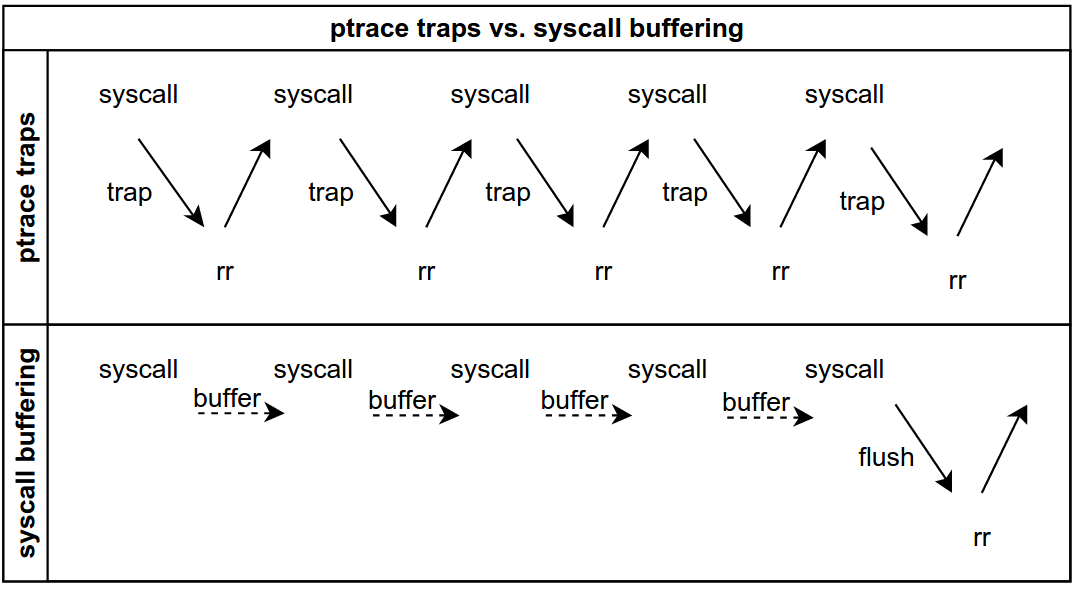
\includegraphics[scale=0.30]{Pictures/png/RR_AS}
\caption[Comparaison de l'exécution du rejeu de RR]{Comparaison de l'exécution du rejeu de RR avec \texttt{ptrace} et seccomp/BPF
  pour gérer l'exécution des appels systèmes.}
\label{AS_RR}
\end{figure}

De par son fonctionnement, RR permet donc de diminuer le temps de débogage. De
plus, il peut fonctionner avec de nombreuses applications puisqu'il arrive à
gérer une grosse application telle que Firefox. Le sur-coût de la phase
d'enregistrement par rapport à un simple debogage avec \texttt{gdb} varie selon les
applications et les tests effectués. Néanmoins, le fait que RR n'enregistre pas
la mémoire partagée en multi-tâche est un problème pour déboguer des threads. De
plus, il émule une machine simplement mono-c\oe ur ce qui est un problème pour
l'utilisation du parallélisme. Tous les appels système ne sont pas encore
implémentés et en fonction de l'application à tester on risque de voir
apparaître un problème d'interception de certains appels système exécutés par
les processus.

\subsection{Distem}
\label{subsection:Distem}
%Partie virtualisation standard

Distem \citep{DISTEM} est un outil libre permettant de construire des
environnements expérimentaux distribués virtuels. Pour cela il fournit un
système de virtualisation de n\oe uds, une émulation des c\oe urs du processeur
de la machine hôte et du réseau. À partir d'un ensemble de n\oe uds homogènes,
il peut émuler une plateforme de n\oe uds hétérogènes connectés via un réseau
lui-même virtuel.

Cet outil qui se veut simple d'utilisation propose différentes interfaces selon
les besoins et les compétences de l'utilisateur. De plus, il supporte
parfaitement le passage à l'échelle puisqu'en 2014, 40 000 n\oe uds ont été
émulés en utilisant moins de 170 machines physiques
\citep{DISTEM_buchert2014emulation}. Le prochain objectif étant de réussir à
émuler 100 000 machines.

Pour construire un environnement distribué virtuel, Distem fait de la
virtualisation par limitation telle que nous l'avons définie dans la section
\ref{section:limitation}. On commence par spécifier la latence et la bande
passante en entrée et en sortie de chaque lien du réseau virtuel. Ensuite, on
définit les performances de chaque n\oe ud émulé. Autrement dit, et comme
représenté sur la Figure \ref{Distem_core}, on alloue à chaque n\oe ud virtuel
un certain nombre de c\oe urs du processeur de la machine physique dont on
pourra controller la fréquence individuellement.

\begin{figure}
  \centering
  \includegraphics[scale=0.70]{Pictures/png/Distem_repartion_coeurs_v1}
  \caption{Répartition des c\oe urs d'un processeur d'une machine hôte entre les différents n\oe uds virtuels qu'elle héberge et émulation de leur puissance en n'utilisant qu'une partie de leur puissance.}
  \label{Distem_core}
\end{figure}
  
On construit ensuite l'environnement de test en plaçant les n\oe uds virtuels
sur une machine physique. Pour que l'environnement de test se rapproche au plus
près de la réalité, Distem peut changer à la volée les paramètres du réseau et
la vitesse de chaque c\oe ur alloué à un n\oe ud virtuel.

\begin{figure}
  \centering
  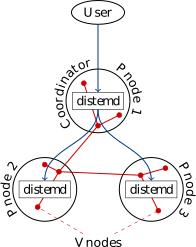
\includegraphics{Pictures/png/Distem_architecture}
  \caption{Architecture de communications de Distem. Ici on a 3 n\oe uds physiques (``Pnodes'') contenant chacun 3 n\oe uds virtuels (``Vnodes'').}
  \label{Distem_archi}
\end{figure}

Comme le présente la Figure \ref{Distem_archi}, Distem repose sur une
architecture simple pour construire son environnement de test distribué virtuel
: les ``Pnodes'' et les ``Vnodes''. Les premiers sont des n\oe uds physiques non
virtualisés alors que les seconds représentent les n\oe uds que l'on souhaite
émuler. Un des Pnodes appelé ``coordinator'' gère le contrôle de
l'infrastructure dans sa globalité en communiquant avec l'ensemble des
Pnodes. Ces derniers peuvent héberger plusieurs Vnodes, chaque Pnode possèdant
son démon Distem qui contrôle les Vnodes. Les Vnodes sont séparés et n'ont pas
connaissance des autres Vnodes présents sur le Pnode. Pour permettre cela,
Distem utilise un conteneur LXC pour émuler un Vnode. Ainsi, chaque Vnode
possède un espace d'adressage séparé pour les ressources sytème (tâches,
interfaces réseau, mémoire...). Néanmoins, les conteneurs LXC partagent
l'utilisation du processeur, ainsi on ne peut pas attribuer un certain nombre de
c\oe urs de CPU à un Vnode. Pour pallier ce problème, Distem utilise en
parallèle \textbf{cgroups} \citep{cgroups}. Pour contrôler la puissance des c\oe
urs attribués à chaque Vnode, Distem utilise l'algorithme
CPU-Hogs\footnote{Méthode de dégradation des performances du CPU qui consiste à
  créer un processus pour qu'il occupe le CPU pendant un certain temps.}
\citep{DISTEM_buchert2011methods}. Ainsi les Vnodes ont connaissance les uns des
autres uniquement via le réseau virtuel. Chaque Vnode possède une ou plusieurs
interfaces réseau virtuelles reliées au réseau physique de l'hôte pour pouvoir
communiquer avec l'extérieur. Du fait du grand nombre de n\oe uds qu'on souhaite
émuler et qui vont communiquer entre eux cet accès au réseau extérieur pose
problème. En effet, pour se reconnaître les n\oe uds vont faire des requêtes ARP
et s'ils sont trop nombreux à envoyer ces requêtes en même temps on va se
retrouver face à un problème d'ARP flooding. La première solution mise en place
par Distem a été d'augmenter la taille des tables ARP pour les Pnodes et les
Vnodes ainsi que l'augmentation du \textit{timeout} d'une entrée dans la
table. Néanmoins, le but de Distem étant de pouvoir émuler de plus en plus de
n\oe uds cette solution finira par ne plus pouvoir s'appliquer. Une autre
solution, qui est celle utilisée actuellement, est de rajouter une couche
d'abstraction réseau à l'intérieur du Pnode en utilisant
VXLAN\citep{VXLAN_mahalingam2014virtual, DISTEM_buchert2014emulation} comme le
montre la Figure \ref{Distem_VXLAN}. Ainsi, les paquets seront échangés entre
Pnodes sur le réseau et c'est la couche VXLAN qui s'occupera d'envoyer au bon
Vnode le paquet reçu sur le Pnode. Ces derniers étant très peu nombreux on est
sûrs de ne pas surcharger les tables ARP.

\begin{figure}
  \centering
  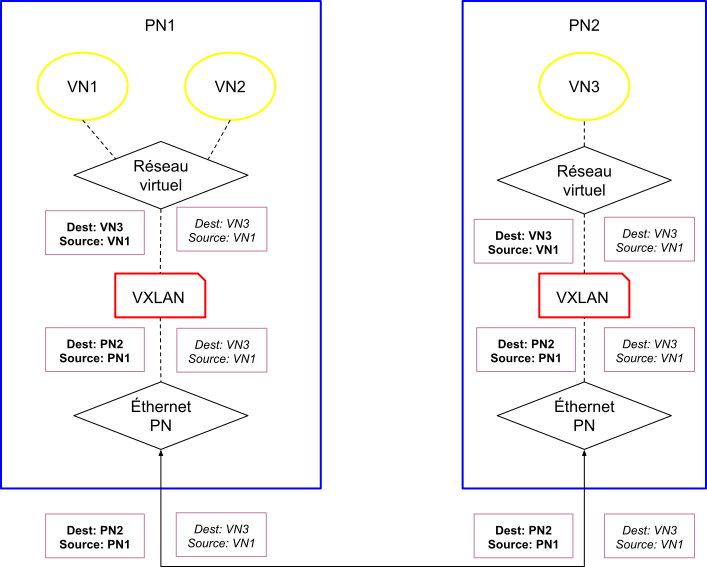
\includegraphics[scale=0.45]{Pictures/png/Distem_VXLAN}
  \caption{Abstraction des communications réseaux de Distem via VXLAN. Les paquets en gras sont ceux envoyés en présence de VXLAN et ceux en italiques sont ceux qui seraient envoyés sur un réseau n'utilisant pas VXLAN.}
  \label{Distem_VXLAN}
\end{figure}

On voit donc que Distem possède une infrastructure et un réseau émulé bien
détaillés et assez réalistes. De plus il est capable de gérer les fautes
injectées au niveau des n\oe uds ou sur le réseau. Son seul problème est donc d'utiliser la virtualisation par limitation empêchant ainsi l'émulation de machines plus puissante que l'hôte.

\subsection{MicroGrid}
\label{subsection:MicroGrid}
MicroGrid \citep{MICROGRID_INIT, MICROGRID_CASANOVA} est un émulateur par interception créé pour résoudre ce problème. Il fournit via l'émulation une grille virtuelle large échelle permettant d'exécuter des applications, sans qu'elles soient modifiées, selon les ressources disponibles sur la grille et les différentes topologies réseau qui peuvent être utilisées par l'application. De plus, la virtualisation permet de gérer toutes les grilles, que leurs ressources soient homogènes ou hétérogènes. Grâce au simulateur, %% utilisé dans la virtualisation par interception, 
MicroGrid peut émuler des machines plus puissantes et donc tester les applications sur des grilles qui n'existent pas encore. En définissant les ressources et le réseau à émuler on peut prédire les performances d'applications développées pour la grille. Le but n'est pas d'avoir des prédictions parfaites mais de parvenir au moins à des estimations de performances qui soient fiables dans le cas de l'exécution d'une application utilisant une topologie inexistante. L'émulateur virtualise l'environnement et le simulateur modélise les ressources de la grille (calcul, mémoire et réseau) pour calculer le temps dans l'environnement virtuel.

Pour maintenir la grille virtuelle, l'émulateur doit gérer deux types de ressources: celles pour le réseau et celles pour le calcul. Dans le premier cas, l'émulateur intercepte toutes les actions faites par l'application qui vont utiliser les ressources simulées (\texttt{gethostname}, \texttt{bind}, \texttt{send}, \texttt{receive}). L'interception se fait au niveau des bibliothèques, via \texttt{LD\_PRELOAD}. Ces appels sont ensuite transmis à l'émulateur de paquets réseau utilisé par MicroGrid, MaSSF, pour gérer les communications qui vont réellement transiter sur le réseau. MaSSF est capable de gérer de très nombreux protocoles réseaux.  Pour ce qui est des ressources de calcul, MicroGrid utilise un contrôleur de CPU qui virtualise les ressources du CPU et gère les processus des machines virtuelles via des \texttt{SIGSTOP} et \texttt{SIGCONT}. Ce contrôleur agit à trois niveaux \textit{i)} il intercepte les appels de fonctions pour créer ou tuer des processus, toujours via \texttt{LD\_PRELOAD}, pour maintenir une table des processus virtuels à jour \textit{ii)} périodiquement il mesure le temps d'utilisation du CPU de chaque processus contenu dans sa table \textit{iii)} il ordonne les processus de chaque hôte virtuel qui sont contenus dans sa table en fonction des mesures qu'il fait.

Dans le cas de grilles hétérogènes il faut obtenir une simulation équilibrée. Autrement dit une simulation qui ne crée pas de délais à cause des temps de réponses qui diffèrent entre les plateformes. Pour cela, il faut mettre en place un mécanisme de coordination globale. MicroGrid utilise un temps virtuel pour coordonner l'écoulement du temps sur les différentes plateformes.

L'avantage de la solution proposée par MicroGrid est qu'elle peut utiliser de nombreux protocoles réseaux complexes pour émuler un réseau réaliste et qu'elle permet d'émuler des machines avec des vitesses très variables grace au contrôleur qui gère la simulation.

Le gros problème de MicroGrid est que le temps n'est pas intercepté mais émulé par dilatation \citep{MICROGRID_lee2014integrated}. Il est très compliqué de trouver le bon facteur de dilatation et de conserver la synchronisation qu'il engendre. De plus, le réseau peut ne pas gérer parfaitement cette dilatation et prendre du retard sur le CPU.

Aujourd'hui il n'existe plus de version maintenue de MicroGrid mais l'approche utilisée par ce projet a été réutilisée dans de nombreux projet notamment Timekeeper\footnote{Permet à chaque conteneur LXC d'avoir sa propre horloge virtuelle et de pouvoir faire des pauses ou des sauts dans le temps. Pour cela la fonction \texttt{gettimeofday} a été réimplémentée afin qu'elle renvoie un temps virtuel.} \citep{MICROGRID_lamps2014timekeeper} et Integrated simulation and émulation using adaptative time dilation\footnote{Ce projet  dilate le temps pour garder une certaine synchronisation entre applications et simulateur. Quand le simulateur est surchargé il prend du retard sur le temps réel et introduit des délais quand il répond à l'émulateur. Ici la fonction \texttt{gettimeofday}() a été remplacée par une \texttt{fonction get\_virtual\_time} et l'émulation se fait par dégradation avec un émulateur type KVM.} \citep{MICROGRID_lee2014integrated}.

\subsection{DETER}
\label{subsection:DETER}

Dans le domaine de la cyber-sécurité, le test de solutions de défenses proposées
face aux différentes menaces n'est pas simple et se développe lentement. En
effet, de nombreuses ressources sont nécessaires et il ne semble pas judicieux
d'effectuer les tests en environnement réel. De plus, les innovations qui
fonctionnent parfaitement dans des environnements contrôlés et prédictibles
sont souvent moins efficaces et fiables dans la réalité de par la taille du
réseau et des ressources qui constituent son environnement.  C'est pour cela que
l'USC\footnote{University Southern California} et l'UC
Berkeley\footnote{Université de Californie à Berkeley} ont lancé le projet DETER
\citep{DETER_Project, DETER_benzel2011science, DETER_mirkovic2010deter}. À sa
création en 2003, DETER était un projet de recherche avancée visant à
développer des méthodes expérimentales pour les innovations en matière de
cyber-sécurité (contrer les cyber-attaques, trouver les failles réseaux
...). Puis en 2004, le besoin de tester ces méthodes se faisant de plus en plus
sentir, le développement de DeterLab\footnote{DeterLab: cyber DEfense Technology
  Experimental Research Laboratory} a été lancé. Cette plateforme d'émulation
par interception libre et partagée fournit un environnement de test large
échelle et réaliste. Elle permet également d'automatiser et de reproduire des
expériences pouvant être de différentes natures. En effet, DeterLab peut
\textit{i)} observer et analyser le comportement de cyber-attaques\footnote{
  Attaques DDos et botnets, vers et codes malicieux, protocoles de stockage
  anti-intrusion (intrusion-tolerant), ainsi que le chiffrement et la détection
  de \textit{pattern}.} et de technologies de cyber-défense, \textit{ii)} tester et
mesurer l'efficacité des solutions de défenses proposées pour contrer les
menaces. Les utilisateurs accèdent aux machines dont ils ont besoins pour leurs
expériences, demandent une certaine configuration du réseau, du système et des
applications présentes sur les machines. Pour fonctionner, ce laboratoire virtuel a
développé 7 outils complémentaires. Seuls 4 outils nous intéressent dans le cadre de notre projet\footnote{Les 3 autres sont le simulateur de comportement humain DASH, ``Multy-party Experiments'' pour avoir une vision partielle du monde lors d'une expérience et ``Risky Experiment Management Capability'' pour gérer les échanges d'expériences avec le réseau extérieur.}.

Le premier, qui constitue le c\oe ur logiciel et hardware de DeterLab, se base
sur Emulab \citep{EMULAB_INIT}. DeterLab a étendu ce dernier pour permettre de
faire des tests large échelle spécialisés dans le domaine de la cyber-sécurité
et dont la complexité est représentative des réseaux d'aujourd'hui (nombre de
n\oe uds, hétérogénéité des plateformes, contrôle de la bande passante et
délai). Il fournit également une interface web pour gérer à distance ses
expériences, les projets en développement et accéder aux autres outils de
DeterLab.

\begin{figure}
  \centering 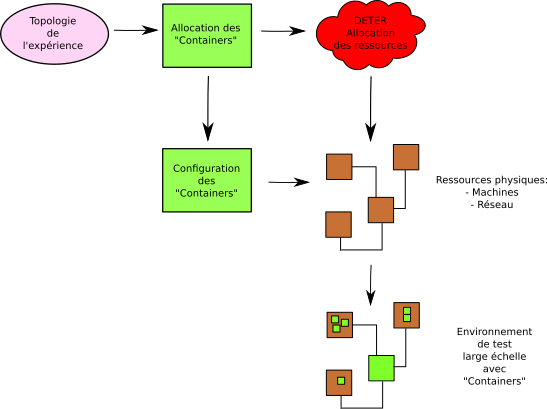
\includegraphics[scale=0.75]{Pictures/png/Deter_fonctionnement_container_v2}
  \caption{Diagramme du fonctionnement d'un \textit{Container}.}
  \label{Conteneur}
\end{figure}

Pour gérer les ressources nécessaires à leurs expériences, les
chercheurs du projet DETER ont créé ``The DeterLab Containers''
(Figure \ref{Conteneur}). Ces derniers permettent de virtualiser les
ressources et donc de répartir la puissance de calcul là où elle est
nécessaire. Ainsi, pour des ressources nécessitant une machine entière,
le conteneur sera la machine alors que pour une ressource qui n'aura
besoin que d'une partie de la machine, le conteneur sera une
abstraction de cette partie de la machine contenant les ressources
utilisées par l'application. Cela permet d'isoler les tests qui
n'utilisent pas une machine complète et de partager ses ressources
entre plusieurs tests concurrents. Ce mécanisme de virtualisation
s'appelle la ``Multi-resolution Virtualization''.

Actuellement, il existe plusieurs plateformes de tests basées sur Emulab avec
des extensions pour pouvoir être utilisées dans des domaines spécifiques comme
le fait DETER. Il se peut qu'une expérience exécutée sur une de ces plateformes
aie besoin de plus de machines que la plateforme ne peut en fournir, que ce soit
en terme de nombre, de puissance ou d'hétérogénéité des machines. Pour pallier
ce problème, le projet DETER a créé la
``Federation''\citep{DETER_faber2007deter}. Elle permet de déployer une
expérience sur plusieurs plateforme de tests différentes et d'avoir un plus
grand facteur de passage à l'échelle. La Figure \ref{Federation} montre
l'exécution d'une expérience dont les 3 n\oe uds sont répartis sur différentes
plateformes. La difficulté ici est que les plateformes sont contrôlées par des
propriétaires différents ayant des règles de sécurité d'accès souvent très
différentes de celles du projet DETER.

\begin{figure}
  \centering 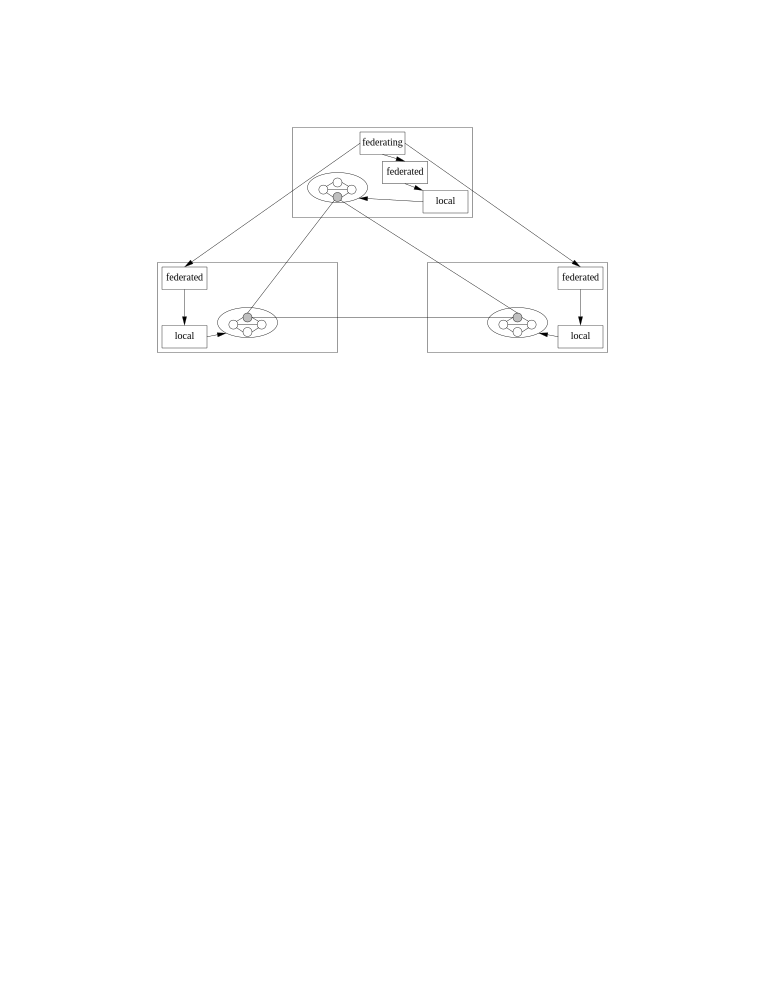
\includegraphics[scale=0.75]{Pictures/png/Deter_federation}
  \caption{Fédération d'une expérience répartie sur 3 plateformes de tests différentes.}
  \label{Federation}
\end{figure}

Pour que cette solution fonctionne, les plateformes vont partager un système de
nommage permettant de ne pas montrer à l'application la répartition de ses
ressources sur le réseau et une authentification pour contrôler l'accès d'une
plateforme à une autre. Pour gérer cela on va utiliser trois types de n\oe uds
différents (Figure \ref{Federation}). Le premier est le ``federating'', il est
unique et se place sur la plateforme qui demande à exécuter une expérience. Il
cherche les ressources disponibles sur les différentes plateformes puis divise
l'expérience en sous-expérience qu'il assigne à chaque plateforme. Il gère
l'exécution de l'expérience, récupère les données à la fin et
libère les ressources utilisées. Le second type de n\oe ud est le ``federated'',
on en place un sur chaque plateforme. C'est lui qui fournit la liste des
ressources disponibles sur sa plateforme de tests et qui configure les
sous-expériences qu'il reçoit du federating. Il fait la traduction de nom entre
le federating, qui utilise le système de nommage partagé, et le réseau local qui
utilise son système de nommage spécifique.  Il gère également la mise en place
des connexions réseaux entre les entités réparties sur les différentes
plateformes. Le dernier n\oe ud appelé ``local'' est également présent sur
chaque plateforme où l'expérience va s'exécuter. Il gère les communications
entre les différentes plateformes et les sécurise pour éviter les fuites à
l'extérieur du réseau ou l'espionnage par d'autres applications s'exécutant sur
la même plateforme.

Pour finir, MAGI\footnote{Montage AGent Infrastructure} fournit un système de
gestion de flux entre les différentes entités d'une expérience, permettant ainsi
d'avoir un certain contrôle sur les machines. En gérant le flux, on peut
automatiser et reproduire les expériences. En effet, MAGI capture chaque
séquence d'instructions concurrentes que l'expérience va suivre pour gérer le
flux, ainsi on peut rejouer la capture plus tard avec les paramètres d'origine
ou des nouveaux si un fichier de paramètres à tester existe. MAGI permet
également de visualiser l'évolution d'une expérience en cours d'exécution pour
s'assurer que son comportement reste correct sans avoir à attendre le résultat
final. En capturant les configurations demandées par les utilisateurs, MAGI
permet leur réutilisation par d'autres utilisateurs pour éviter à DETER de
reconstruire la même architecture pour une prochaine expérience.

\begin{figure}[H]
\centering
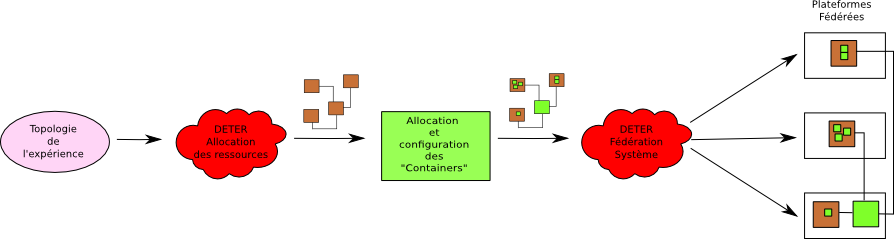
\includegraphics[scale=0.63]{Pictures/png/Deter_fonctionnement_general}
\caption{Création de l'environnement d'une expérience.}
\label{Deter_fonc}
\end{figure}

 Actuellement, DeterLab peut émuler des dizaines de milliers de n\oe uds: le
 projet dispose de 500 machines et 10 FPGA. Il est le seul émulateur dans le
 domaine de la cyber-sécurité et permet de faire des tests large échelle dont la
 complexité est représentative des réseaux.

%% \subsection{ROBOT}


\newpage
\section{Simterpose: la médiation}
\label{section:simterpose}

Dans la section précédente, nous avons présenté différents projets permettant de faire de la virtualisation légère. Malheureusement, ils ne pouvaient pas être
utilisés dans le cadre de notre projet. Nous allons donc voir pourquoi et quel
est l'émulateur qui a été choisi pour permettre d'exécuter des applications
distribuées au dessus de SimGrid. Puis, nous étudierons le fonctionnement interne de
cet émulateur, notamment les outils présentés en section \ref{section:tools}
qu'il utilise.

\subsection{Organisation générale}
%schéma tableau

Dans le cadre du projet Simterpose de virtualisation légère et de test
d'applications distribuées, c'est l'émulation par interception qui a été
choisie. En effet, le but final étant de pouvoir évaluer n'importe quelle
application distribuée sur n'importe quel type d'architecture, on peut se
retrouver à devoir émuler des machines plus puissantes que l'hôte, ce que
l'émulation par dégradation ne permet pas. Ce choix exclut donc l'utilisation de
Distem dans notre projet. Les autres outils de virtualisation par interception
ont été écartés pour des raisons différentes: CWRAP utilise uniquement
\texttt{LD\_PRELOAD} pour intercepter les actions et est spécifique aux
applications réseau. RR gère le multithread mais pas la virtualisation réseau. MicroGrid utilise une émulation par dilatation pour gérer le temps. Or, dans notre cas, nous voulons faire de l'interception. Pour finir, nous avons écarté le projet DETER car il est limité au domaine de la cyber-sécurité.

Pour satisfaire les besoins de notre projet, il a été décidé de créer un nouvel
émulateur Simterpose. Ce dernier doit être simple d'utilisation et facilement
déployable (simple ordinateur ou cluster).  De plus, il doit permettre
d'exécuter plusieurs instances d'une application sur une même machine et de proposer une large gamme de conditions d'exécutions (simple n\oe ud ou réseau
complexe). Les expériences devant être reproductibles, l'émulateur doit pouvoir
générer des traces pour les rejouer dans le simulateur. La résistance aux
pannes, et le fait de pouvoir fonctionner sans avoir accès au fichier source de
l'application sont également des conditions à satisfaire.

Simterpose utilise la plateforme de simulation SimGrid, dont l'architecture est
représentée Figure \ref{SimGrid}, pour générer l'environnement virtuel
nécessaire à l'expérience. À sa création en 1999, SimGrid était une plateforme
fournissant des outils pour construire un simulateur afin d'étudier les
algorithmes d'ordonnancement en environnement hétérogène, puis il a évolué \citep{casanova:hal-01017319} pour devenir plus générique. Aujourd'hui, c'est
devenu une plateforme de simulation permettant d'évaluer les applications
distribuées large échelle s'exécutant dans des environnements hétérogènes.
 
\begin{figure}[H]
  \centering
  \includegraphics[scale=0.95]{Pictures/png/SimGrid}
  \caption{Architecture de la plateforme SimGrid}
  \label{SimGrid}
\end{figure}

La Figure \ref{Organisation_generale} présente l'organisation générale de la plateforme de simulation. SimGrid va générer l'environnement virtuel. Simterpose intercepte les
actions de l'application et les modifie pour maintenir l'émulation si
nécessaire. Puis, il les laisse
s'exécuter sur la machine hôte et va interroger SimGrid pour qu'il calcule la
réponse de l'environnement virtuel aux actions de l'application (temps d'exécution, gestion de communications réseau). La Figure \ref{Organisation_Simterpose} illustre ce fonctionnement.

\begin{figure}[H]
  \centering
  %\includesvg{Pictures/svg/Communications_Simterpose_interprocess_v2}
  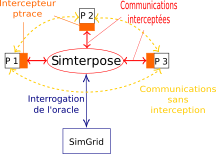
\includegraphics{Pictures/png/Communications_Simterpose_interprocess_v2}
  \caption{Architecture de communication entre les différents acteurs}
  \label{Organisation_generale}
\end{figure}

\begin{figure}[H]
  \centering
  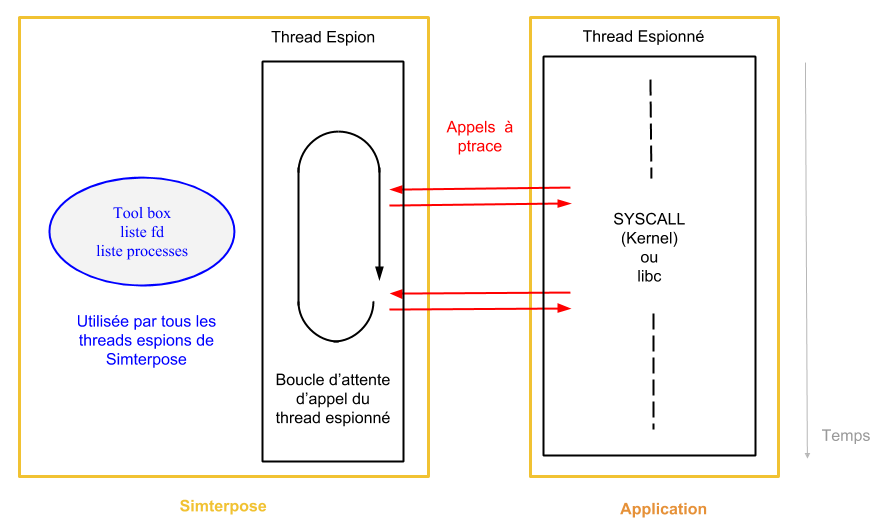
\includegraphics[scale=0.5]{Pictures/png/Simterpose_orga_code_v4}
  \caption{Le fonctionnement de Simterpose}
  \label{Organisation_Simterpose}
\end{figure}

Maintenant que nous avons présenté le cadre général et l'organisation globale
de notre projet, nous allons nous intéresser au fonctionnement de Simterpose.

\subsection{Fonctionnement interne de Simterpose}
\label{subsection:fonctionnement_simterpose}

Les actions à intercepter pour maintenir la virtualisation sont de différentes
natures. Il peut s'agir d'actions liées aux communications réseaux, à la
création et à l'identification des processus, à la gestion du temps, ainsi qu'à
l'utilisation du protocole DNS. Pour chacune, les outils utilisés ne sont pas
nécessairement les mêmes. Nous allons donc voir lesquels sont employés parmi
ceux cités dans la section \ref{section:tools}.

\subsubsection{Les communications réseaux}
 %-> syscall -> ptrace (full mediation, address translation)
\label{subsubsection:fonctionnement_reseau}

Dans le cas d'une communication réseau, le but de Simterpose étant de réussir à
simuler un réseau virtuel sur un réseau local, il faut gérer la transition entre
réseau local et réseau simulé, comme le montre la Figure \ref{COMM}. En effet,
l'application possède une adresse IP et des numéros de ports virtuels qui ne
correspondent pas à ceux attribués dans le réseau local.

La gestion de cette transition va se faire au niveau des appels systèmes, car nous ne souhaitons pas oublier des fonctions en utilisant \texttt{LD\_PRELOAD}. Pour intercepter les appels systèmes liés au réseau nous allons utiliser l'appel système \texttt{ptrace} présenté en section \ref{subsection:ptrace}.

\begin{figure}[H]
  \centering
  \begin{subfigure}{0.5\textwidth}
    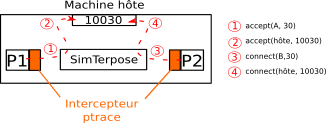
\includegraphics[scale=0.8]{Pictures/png/Mediation_realite}
    \caption{Communications réelles}
  \label{COMM_REALITE}
  \end{subfigure}
  \begin{subfigure}{0.25\textwidth}
  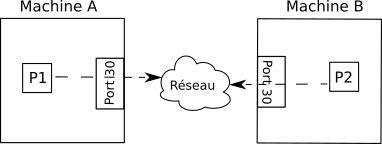
\includegraphics[scale=0.5]{Pictures/png/Mediation_VM}
  \caption{Communications vues \\ par les processus}
  \label{COMM_VM}
  \end{subfigure}
  \caption{Les communications réseau entre deux processus}
  \label{COMM}
\end{figure}

De plus, il n'est pas suffisant de se baser uniquement sur le descripteur de fichier associé à une socket pour identifier deux entités qui communiquent
entre elles. En effet ce descripteur est unique pour chaque socket
d'un processus, mais plusieurs processus peuvent avoir un même descripteur de fichier pour des sockets de communications différentes puisque
chacun à son propre espace mémoire. Pour pallier à ce problème, nous allons utiliser les adresses IP et les ports locaux et distants des
deux entités qui souhaitent communiquer comme moyen d'identification en plus du numéro de socket.

Afin de gérer toutes ces modifications deux solutions ont été proposées lors
d'un précédent stage \citep{GUILLAUME:Interceptionsyscall}: l'\textit{address
  translation} et la \textit{full mediation}. Néanmoins, ces deux solutions
n'ont pas encore été évaluée en pratique.
 
\paragraph{Traduction d'adresse}
 Avec ce type de médiation, illustrée Figure \ref{ADDRESS_TRANSLATION}, on laisse le noyau gèrer les communications. Ainsi, en entrée et sortie d'appel système, Simterpose va juste s'occuper de la transition entre le réseau virtuel simulé
 par SimGrid et le réseau local, en utilisant les informations de communications
 contenues dans la socket. Pour cela, Simterpose gère un tableau de
 correspondances, dans lequel pour chaque couple <IP, ports>virtuels , on a un
 couple <IP, ports>réels associé.  De fait, en entrée d'un appel système de
 type réseau (\texttt{bind}, \texttt{connect}, \texttt{accept} ...), Simterpose
 doit remplacer l'adresse et les ports virtuels de l'application par l'adresse
 et les ports réels sur le réseau local, afin que la source de l'appel système
 corresponde à une machine existante sur le réseau local. Au retour de l'appel
 système, il faudra remodifier les paramètres en remettant l'adresse et les
 ports virtuels. La limite de cette approche est liée au nombre de
 ports disponibles sur l'hôte.

\paragraph{Full mediation} \label{paragraph:FULL_MEDIATION}
Dans ce cas, le noyau ne va plus gérer les communications car nous allons
empêcher l'application de communiquer via des sockets et même d'établir des
connexions avec une autre application. Puisqu'il n'y a aucune communication, on
n'a pas besoin de gérer de tableau de correspondance d'adresses et de ports et
les applications peuvent conserver les adresses et les ports simulés qu'elles
considèrent comme réels. Quand l'application voudra faire un appel système de
type communication ou connexion vers une autre application, le processus espion
de Simterpose qui sera notifié via \texttt{ptrace} neutralisera l'appel système,
comme illustré sur la Figure \ref{FULL_MEDIATION}. Ensuite, ce processus
récupérera, en lisant dans la mémoire du processus espionné, les données à
envoyer ou récupérer et ira directement les lire ou les écrire dans la mémoire
du destinataire.

\begin{figure}[H]
   \centering
   \begin{subfigure}{0.5\textwidth}
   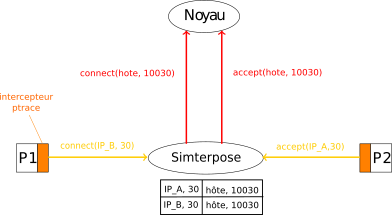
\includegraphics[scale=0.5]{Pictures/png/Mediation_translation_v2}
   \caption{\textit{Address translation}}
   \label{ADDRESS_TRANSLATION}
   \end{subfigure}
   \begin{subfigure}{0.4\textwidth}
     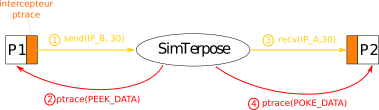
\includegraphics[scale=0.5]{Pictures/png/Mediation_full_v2}
  \caption{\textit{Full mediation}}
  \label{FULL_MEDIATION}
   \end{subfigure}
   \caption{Les différents types de médiation}
   \label{MEDIATION}
 \end{figure}

\subsubsection{Les threads}
 %% syscall clone + libcalls

La gestion des threads se fera à deux niveaux dans Simterpose. On fera appel à l'interception d'appels système via \texttt{ptrace} pour tout ce qui concerne la création de threads (\texttt{fork}, \texttt{clone}, \texttt{pthread\_create}). Pour le reste on utilisera un autre outil, car certains mécanismes utilisés par les threads ne passent pas par des appels systèmes pour s'exécuter, par exemple les futex\footnote{Fast User-space mutex \url{http://man7.org/linux/man-pages/man7/futex.7.html}}. On utilise donc le préchargement de bibliothèques dynamiques en complément. Comme nous l'avons vu en section \ref{paragraphe:LDPreload}, nous allons créer une librairie contenant toutes les fonctions utilisées par les threads que nous voulons intercepter (\texttt{pthread\_init}, \texttt{pthread\_join}, \texttt{pthread\_exit}, \texttt{pthread\_yield} ...). On placera ensuite la bibliothèque dans la variable d'environnement \texttt{LD\_PRELOAD} pour que nos fonctions passent avant les autres.



\subsubsection{Le temps}
\label{subsubsection:time}
%% -> syscall (- system wide), VDSO-linker (cross process ou VDSO)

Nous souhaitons que l'écoulement du temps perçu par les applications soit un
temps virtuel, celui qui s'écoulerait dans l'environnement simulé, pour que
l'émulation soit plus réaliste. Il y a deux types d'actions à différencier pour
gérer le temps: les appels de fonctions liées au temps et les actions faites par
l'application qui prennent du temps lors de leur exécution.

Dans le premier cas, Simterpose va intercepter les appels de fonctions
temporelles et les modifier pour renvoyer l'horloge virtuelle. Ces dernières étant
assez nombreuses, il est moins coûteux, en terme charge de travail pour
le programmeur, d'intercepter via
\texttt{ptrace} les appels sytèmes temporels (\texttt{time},
\texttt{clock\_gettime}, \texttt{gettimeofday}).

Néanmoins, il a été montré dans un précédent stage \citep{CHLOE:Emulationapplicationdistribuees} que \texttt{ptrace} est inefficace
voire inutile en ce qui concerne l'interception des appels systèmes temporels
qu'une application souhaiterait exécuter car le noyau ne les exécute pas. Cela
est dû à l'existence de la bibliothèque \textit{Virtual Dynamic Shared Object}
(\texttt{VDSO}). Cette dernière vise à minimiser les coûts dûs aux deux changements de contexte effectués lors de l'exécution d'un appel système. \texttt{VDSO} va retrouver l'heure dans un segment du processus partagé avec l'espace noyau lisible par tous les processus sans changer de mode. Il est possible de désactiver cette bibliothèque lors du boot mais cela réduit les performances, augmente le nombre de changements de contexte, et oblige l'utilisateur à modifier les paramètres de son noyau.

On va donc se placer à un autre niveau pour intercepter ces
fonctions. Malgré leur nombre, il a été décidé d'agir lors du
préchargement de bibliothèque. On va créer une bibliothèque qui
surcharge les appels de fonctions liées au temps et la placer dans la
variable d'environnement \texttt{LD\_PRELOAD}. Une fois l'interception
temporelle effectuée, Simterpose interroge SimGrid pour obtenir
l'horloge virtuelle et la renvoie à l'application.

Dans le second cas, lors d'une action interceptée (calcul, communications
réseau), Simterpose doit gérer l'horloge de l'application avant de lui renvoyer
le résultat de l'exécution. Pour cela, Simterpose envoie à SimGrid l'heure et la
durée d'exécution sur la machine hôte. Ce dernier calcule en fonction de ces
deux informations, le temps qui aurait été nécessaire pour une telle exécution
sur la plateforme virtuelle et l'envoie à Simterpose. Pour finir, l'émulateur
rend la main à l'application en lui envoyant l'heure virtuelle en plus du
résultat de son action.

\subsubsection{DNS}
 \label{section:DNS}
%% libcalls (ne rien rater), config fake (system wide), intercept 53 ( plus dur que nécessaire, port dns autre ou pas)

Dans le cas d'utilisation du protocole DNS, on peut vouloir modifier le
comportement de l'application afin qu'elle utilise d'autres serveurs que ceux
utilisés par défaut, ou aucun afin que la résolution soit entièrement gérée par
Simterpose. 

Une première solution envisageable serait de faire de l'interception de
communications au niveau du port 53, utilisé par défaut dans DNS. Néanmoins,
cela est assez complexe à mettre en \oe uvre car il faut pour chaque
communication faite par l'application tester le port qu'elle souhaite
utiliser. De plus, il est possible que l'utilisateur définisse un autre port
pour le protocole DNS que celui par défaut. Cette solution n'est donc pas
suffisante.

Une autre approche serait de remplacer le fichier \texttt{resolv.conf}
utilisé pour la résolution de nom par un fichier spécifié par
l'utilisateur. Il pourrait également fournir un fichier de
spécification de comportement en cas d'utilisation de DNS permettant
à Simterpose de générer un nouveau
fichier \texttt{resolv.conf}. Néanmoins, cette solution génère une
surcharge de travail pour l'utilisateur et nous souhaitons avoir un
émulateur qui soit simple d'utilisation.

La dernière solution envisageable est de faire de l'interception d'appel de
fonctions. Dans ce cas, on créé une bibliothèque partagée qui réécrit les fonctions
liées à la résolution de nom que l'on inclut dans la variable d'environnement
\texttt{LD\_PRELOAD}. Mais on a toujours le même problème qui est de n'oublier
aucune fonction pour maintenir notre environnement virtuel. Pour l'instant,
c'est la solution qui a été choisie. N'ayant pas encore été mise en place, il
n'est pas exclu que nous devions trouver une autre solution pour gérer le DNS.

\vspace{0.5cm}

Dans cette section, nous avons étudié l'organisation globale de Simterpose ainsi
que son fonctionnement interne. Nous avons pu voir que deux des outils présentés
en section \ref{section:tools} sont utilisés pour implémenter notre émulateur:
l'appel système \texttt{ptrace} et la variable
d'environnement \texttt{LD\_PRELOAD}.



\newpage
\section{Travail réalisé}

Au cours de ce stage, deux des fonctionnalités majeures de Simterpose présentées en section \ref{subsection:fonctionnement_simterpose} ont été implémentées: le réseau de communications et la gestion du temps. Ces fonctionalités ont parfois nécessité la mise en place de nouveaux outils. De plus, plusieurs améliorations ont été apportées à notre émulateur. Dans cette section, nous allons présenter les deux fonctionnalités implémentées ainsi que les outils qu'elles ont nécessités et les améliorations apportées.




\subsection{Réseau de communications}
\label{subsection:network_implementaion}

Afin d'implémenter le réseau de communications, tel qu'il est présenté en section \ref{subsubsection:fonctionnement_reseau}, nous avons écrit pour chaque appel affectant le réseau une version de l'appel utilisant l'\textit{address translation} et une utilisant la \textit{full mediation}. Une des deux versions sera exécutée par \texttt{ptrace} à chaque interception de l'appel selon le type de médiation utilisée.

Dans le cas de l'\textit{address translation}, nous allons récupérer via \texttt{ptrace} les valeurs contenues dans les registres. Ensuite, selon le type d'appel système réseau dont il s'agit, on effectue des actions différentes. Pour les appels qui concernent la création de sockets ainsi que l'ouverture et la fermeture de connexion (\texttt{socket}, \texttt{bind}, \texttt{connect}, \texttt{listen}, \texttt{accept}, \texttt{shutdown}, \texttt{close}) on crée dans la table de correspondance <IP, port>$_{virtuel}$ / <IP, port>$_{\text{réel}}$ un nouvelle entrée, si elle n'existe pas déjà. Cela nous permettra de maintenir la virtualisation en traduisant les couples <IP, port>$_{virtuel}$ en <IP, port>$_{\text{réel}}$ lors d'appels systèmes effectuant des communications sur le réseau. Pour les appels concernant les échanges de messages, on récupère en utilisant les tables de traductions le couple  $<IP, port>_{\text{réel}}$ correspondant aux informations passée en paramètre. Pour finir, quelque soit l'appel système, on va écrire dans ses registres les valeurs traduites grâce à \texttt{ptrace}. Puis, on laisse l'appel système s'exécuter. À la sortie, on refait la même chose à la seule différence qu'on traduit le couple  <IP, port>$_{reel}$ en <IP, port>$_{virtuel}$.

Pour la version de l'appel système qui utilise la \textit{full mediation}, on récupère comme précédement les paramètres de l'appel système contenus dans les registres. Dans cette médiation il est nécessaire d'empêcher les appels systèmes de s'exécuter. On neutralise donc l'appel système via \texttt{ptrace} pour empêcher son exécution quand on rendra la main à l'application. Puis, en fonction du type d'appel système réseau on effectue différentes actions. Aucune action n'est nécessaire pour les appels qui concernent la gestion du réseau (création de socket, ouverture et fermeture de connexion...) puisque dans ce type de médiation aucune socket n'est créée et connectée. Pour les appels systèmes qui vont effectuer des échanges de messages, on crée une tâche SimGrid qui va permettre d'écrire ou de lire les données à envoyer ou recevoir. Puis, pour tous les types d'appels systèmes réseau, on écrit dans les registres de l'appel avec \texttt{ptrace}: la valeur de retour de l'appel et éventuellement d'autres informations dans différents registres selon l'appel. C'est le cas par exemple, quand on reçoit des données: elles sont lues durant l'exécution de l'appel système par le noyau. Elles sont ensuite écrites dans le buffer d'écriture dont l'adresse est passée en paramètre.

\subsection{Temps}
\label{section:work:time}

Pour pouvoir maintenir notre environnement virtuel, nous avons expliqué en section \ref{subsubsection:time} que nous ne pouvons pas laisser les applications accéder aux horloges de la machine hôte, utilisant pour cela la bibliothèque \texttt{VDSO}. Nous avons alors proposé de créer une bibliothèque réimplémentant les fonctions temporelles et d'utiliser la variable d'envieronnement \texttt{LD\_PRELOAD}, présentée en section \ref{paragraphe:LDPreload}, pour exécuter les fonctions de notre bibliothèque en priorité. De cette façon, on bloque les appels à la bibliothèque \texttt{VDSO} et l'application ne peut plus accéder au temps de la machine hôte. Néanmoins, pour que notre virtualisation soit parfaite il faudrait que le temps que l'applicatioin voit s'écouler soit celui qui s'écoulerait sur la machine simulée par SimGrid. 

Pour permettre cela, nous avons créé une bibliothèque de fonctions temporelles que nous plaçons dans la variable d'environnement \texttt{LD\_PRELOAD} à chaque exécution d'une application avec Simterpose. Cette bibliothèque contient pour chaque fonction de la \texttt{libc} qui fasse appel à une des horloges de la machine (\texttt{ftime}, \texttt{time}...) une nouvelle fonction de même prototype. Maintenant, au lieu de demander l'horloge de la machine hôte, les nouvelles fonctions de temps demandent à SimGrid de fournir l'heure sur la machine qu'il est en train de simuler. Comme le montre la figure \ref{}, l'appel à la fonction de temps se fait dans l'application qui s'exécute sur le thread "espionné" de Simterpose. Ce dernier est controlé par le processus 'espion' via l'intercepteur \texttt{ptrace} qui est le seul processus de Simterpose à pouvoir communiquer avec le simulateur. Nous devons donc passer par le thread "espion" pour pouvoir interrroger SimGrid. 

{\color{red} pas clair}
\textit{Cependant, le seul moyen de faire intervenir le processus "espion" est d'effectuer un appel système dans l'application en train de s'exécuter. Dans notre cas, c'est la nouvelle fonction temporelle qui doit effecteur l'appel système. En effet, le processus "espion" va intercepter l'appel et exécuter le "handler" qu'on lui aura fourni si nécessaire, comme pour le reseau de communications, avant de rendre la main à l'application en plaçant dans le registre de retour de l'appel système l'horloge que lui aura donné le simulateur. Si une autre fonction effectue l'appel, la nouvelle fonction temporelle ne pourra pas récupérer la valeur de retour de l'appel système et ainsi retourner l'heure simulée à l'application. De plus, puisque nous souhaitons juste récupérer l'horloge de l'environnement virtuel et rien d'autre, il faudra que le "handler" que va exécuter \texttt{ptrace} avant l'appel contienne l'appel à la fonction \texttt{MSG\_get\_clock}, qui permet de récupérer l'heure dans SimGrid et neutralise l'appel système choisit avant de rendre la main à l'application. 
}

Néanmoins, la fonction temporelle ne doit pas utiliser n'importe quel appel système pour récupérer l'heure simulée. Par exemple, si on choisit de modifier l'appel système \texttt{send}, on va placer dans le handler de ce dernier l'appel à la fonction \texttt{MSG\_get\_clock} puis on le neutralise. Or, lorsqu'on voudra utiliser cet appel système pour envoyer des données sur le réseaux on ne pourra plus le faire car l'intercepteur \texttt{ptrace} exécutera le nouveau handler et l'appel ne sera plus exécuté. Il nous faut donc trouver un appel système dont on n'aura jamais besoin pour faire autre chose que récupérer l'heure simulée. Dans tous les noyaux, il existe des appels systèmes qui ne sont plus implémentés; c'est le cas de l'appel système \texttt{tuxcall}. Quand on fait appel à ce dernier le système ne fait rien, il émet juste un avertissement pour dire que l'appel n'existe plus. Nous avons donc choisi de placer notre handler sur cet appel système.

Les Figures \ref{TODO}, \ref{TODO} et \ref{TODO} nous montrent respectivement l'algorithme de la nouvelle fonction \texttt{time}, le handler de l'appel système \texttt{tuxcall}, et ce qui se passe dans SimGrid et Simterpose quand on veut récupérer l'heure simulée grâce à la double interception complémentaire de \texttt{LD\_PRELOAD} et \texttt{ptrace}.



\subsection{Améliorations apportées à Simterpose}

Au début de ce stage, Simterpose ne pouvait être exécuté que sur des architectures 64bits. Considérant qu'il est important qu'un tel programme puisse s'exécuter sur tous les types d'architecture nous avons voulu résoudre ce problème afin qu'il puisse s'exécuter sur des machines 32bits. Il existe plusieurs différences entre les architectures 32bits et 64bits. Celles qui nous intéressent sont celles qui sont susceptibles d'affecter Simterpose. La première différence est que les registres ne portent pas les mêmes noms en 64bits et 32bits, cf tableau \ref{register}. Or, lorsqu'on intercepte des appels systèmes il faut pouvoir récupérer les valeurs contenues dans les registre à l'entrée de l'appel système puis écrire dans ces mêmes registres à la sortie. Afin d'exécuter Simterpose sur ces deux architectures il faut donc avoir une version du code pour chacune. Chaque version utilisant les bons noms de registres pour récupérer les valeurs qu'ils contiennent lors de l'interception d'appels systèmes via \texttt{ptrace}. Pour trouver sur quelle type de plateforme Simterpose est en train de s'exécuter on teste la valeur maximale que peut avoir un pointeur en mémoire avec la \texttt{macro} \texttt{UINTPTR\_MAX}. Pour avoir une architecture 64bits UINTPTR\_MAX doit valoir 0xffffffffffffffff et pour être en 32bits elle doit valoir 0xffffffff. La seconde différences est que certaines \texttt{macro} et appels systèmes n'existent pas sur des architectures 64bits et inversement. C'est la cas de deux appels systèmes particulièrement importants car ils touchent au réseau: \texttt{send} et \texttt{recv}. Ces deux appels ne sont définis que pour des architectures 32bits, sur des architectures 64bits quand on les utilise ils sont remplacés par les appels sytèmes \texttt{sendto} et \texttt{recvfrom}.

\begin{table}[]
\centering
\begin{tabular}{lcccccccc}
\cline{2-9}
\multicolumn{1}{l|}{}              & \multicolumn{1}{c|}{{\bf \begin{tabular}[c]{@{}c@{}}Numéro de\\ l'appel système\end{tabular}}} & \multicolumn{1}{c|}{{\bf \begin{tabular}[c]{@{}c@{}}Valeur \\ de retour\end{tabular}}} & \multicolumn{1}{c|}{{\bf arg0}} & \multicolumn{1}{c|}{{\bf arg1}} & \multicolumn{1}{c|}{{\bf arg2}} & \multicolumn{1}{c|}{{\bf arg3}} & \multicolumn{1}{c|}{{\bf arg4}} & \multicolumn{1}{c|}{{\bf arg5}} \\ \hline
\multicolumn{1}{|c|}{{\it 32bits}} & \multicolumn{1}{c|}{orig\_eax}                                                                 & \multicolumn{1}{c|}{eax}                                                               & \multicolumn{1}{c|}{edi}        & \multicolumn{1}{c|}{esi}        & \multicolumn{1}{c|}{edx}        & \multicolumn{1}{c|}{r10d}       & \multicolumn{1}{c|}{r8d}        & \multicolumn{1}{c|}{r9d}        \\ \hline
\multicolumn{1}{|c|}{{\it 64bits}} & \multicolumn{1}{c|}{orig\_rax}                                                                 & \multicolumn{1}{c|}{rax}                                                               & \multicolumn{1}{c|}{rdi}        & \multicolumn{1}{c|}{rsi}        & \multicolumn{1}{c|}{rdx}        & \multicolumn{1}{c|}{r10}        & \multicolumn{1}{c|}{r8}         & \multicolumn{1}{c|}{r9}         \\ \hline
                                   & \multicolumn{1}{l}{}                                                                           & \multicolumn{1}{l}{}                                                                   & \multicolumn{1}{l}{}            & \multicolumn{1}{l}{}            & \multicolumn{1}{l}{}            & \multicolumn{1}{l}{}            & \multicolumn{1}{l}{}            & \multicolumn{1}{l}{}           
\end{tabular}
\caption{Nom des différents registres d'un appel système selon le type d'architecture.}
\label{register}
\end{table}

La seconde amélioration est une mise à niveau de Simterpose pour qu'il puisse utiliser les dernières version de SimGrid. Pour cela, il a fallu remplacer d'anciennes fonctions et variables encore utilisées dans le code de Simterpose par les nouvelles utilisées dans SimGrid. Cela a également permi de mettre à jour un problème dans SimGrid dû à l'accès d'un pointeur dont on ne vérifiait pas qu'il n'était pas nul. Au début de mon stage, Simterpose utilisait une version de SimGrid datant de 2011, maintenant il utilise la version f42adf1 de git sortie le 16 Août 2015.

Troisièmememnt, nous souhaitons pouvoir utiliser un autre débugueur en plus de \texttt{gdb}. Nous avons choisi Valgrind pour les nombreux modules qu'il fourni,cité en section \ref{subsubsection:valgrind}, notamment \texttt{memcheck} qui est pour nous le plus intéressant. Ce dernier traque les fuites mémoires et résume en fin d'exécution tout ce qui a été réservé, libérée et perdu en mémoire. Pour permettre son utilisation avec Simterpose nous avons dû implémenter l'appel système \texttt{fcntl}. Valgrind utilise cet appel système pour accéder à l'exécution de Simterpose et ainsi chercher les fuites mémoires. L'implémentation d'un handler pour cet appel n'était pas prévu à la création de Simterpose puisque nous souhaitons juste intercepter les appels systèmes réseaux, temporels et gérer les processus et leurs threads pour maintenir notre environnement virtuel et aucun débugueur autre que \texttt{gdb} ne souhaitait être utilisé à ce moment-là.

Pour finir, le but de Simterpose étant d'exécuter des applications distribuées large échelle, nous devons pouvoir exécuter des applciations de Torrent. De fait, lorsqu'on exécute des applications de ce type, le système de fichier de la machine hôte est en permanence utilisé. Simterpose dispose en parallèle de son propre système de fihier. Pour chaque socket ou fichier il dispose d'un descripteur avec des compteurs de références, les processus qui les référencent, les verrous qui peuvent être posés... Nous devons donc nous aussi maintenir à jour notre système de fichier dans le cas où nous lancerions ce genre d'applications. Ainsi, nous devons maintenant intercepter les appels systèmes touchant aux fichiers en plus de ceux affectant le réseau en utilisant toujours \texttt{ptrace}. Lorsqu'on les intercepte il faut récupérer les modifications qui seront effectués sur le système de fichiers réel une fois qu'on aura laisser passer l'appel système et les appliquer au système de fichier propre à Simterpose. Actuellement Simterpose gére les appels systèmes: \texttt{open},  \texttt{close}, \texttt{creat}, \texttt{dup}, \texttt{dup2}, \texttt{poll}, \texttt{fcntl}, \texttt{lseek}, \texttt{read}, \texttt{write}.

\vspace{0.5cm}


\newpage
\section{Évaluation expériementale}
\label{section:evaluation}

Dans la section précédente, nous avons présenté le travail réalisé au cours de ce stage. Maintenant, nous souhaitons évaluer les performances des fonctionnalités que nous avons implémentées. Pour cela, nous allons d'abord présenter l'architecture utilisée. La plateforme sur laquelle nous avons effectuée nos expériences possède les caractéristiques suivantes: distribution ubuntu 3.13.0-62, Processeur: 4 c\oe urs multithread à 2.60 GHz. En ce qui concerne SimGrid et Simterpose, les commits utilisés pour les expériences sont respectivement f42adf1 (16 Août 2015) et 77f7d81 (19 Août 2015). 

Au niveau de la plateforme réseau simulée par SimGrid on a quatres n\oe uds réliés les uns aux autres. Chaque n\oe ud a une puissance de 10 MFlops, une bande passante de 10 Go/s et une latence de $5.10^{-4}$s. Pour nos expériences on utilise seulement deux de ces n\oe uds, dont l'un joue le rôle de client et l'autre joue le serveur. 

\subsection{Réseau}
\label{subsection:res}

Dans les sections \ref{subsubsection:fonctionnement_reseau} et \ref{subsection:network_implementaion}, nous avons présenté l'organisation et l'implémentation du réseau de communications de Simterpose. Nous voulons maintenant évaluer les performances de notre implémentation à travers divers tests.

\subsubsection{Protocole expérimental}
L'objectif principal étant de montrer qu'il est possible de faire de la virtualisation légère, nous souhaitons d'abord mesurer l'\textit{overhead} dû à l'utilisation de Simterpose. Dans un second temps, nous souhaitons mesurer les performances des deux types de médiations que nous avons implémentés. Cela nous permettrait de savoir quel type de médiation est le mieux adapté à l'application que nous voulons exécuter.

Pour effectuer nos expériences, nous avons choisi deux applications réseau d'échanges de messages. La première application consiste à faire communiquer un client et un serveur en envoyant au serveur un million de messages de petite taille. On en envoie un million pour pallier le manque de précisions des \textit{timers}. La seconde va envoyer depuis un client un message de 1Mo à un serveur. Le protocole pour chaque expérience a été d'exécuter 20 fois chaque application en utilisant les mêmes appels systèmes pour communiquer les messages (\texttt{sendto}/\texttt{recvfrom} et \texttt{sendmsg}/\texttt{recvmsg}), puis une moyenne du temps d'exécution ainsi qu'une mesure des temps minimum et maximum ont été calculés.

\subsubsection{Résultats}
\paragraph{Overhead concernant le temps d'exécution}
Afin de mesurer l'\textit{overhead} produit par Simterpose, notre expérience consiste à exécuter les deux applications réseaux choisies sur une machine en utilisant uniquement le réseau local puis en utilisant Simterpose en suivant le protocole présenté plus haut. Ainsi, en comparant les temps d'exécution des applications sur les deux types d'architecture nous pourrons calculer l'\textit{overhead}. Les résultats de ces expériences sont présentés Figures \ref{Network_Big_Local} et \ref{Network_Little_Local}. L'histogramme représentant Simterpose correspond à la moyenne de 20 mesures en \textit{full mediation} avec 20 mesures en \textit{address translation}.

\begin{figure}[H]
  \centering
    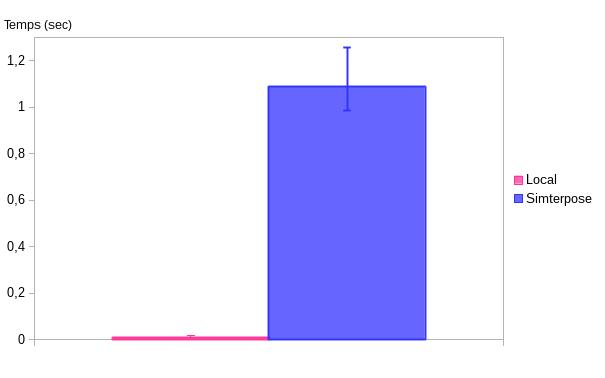
\includegraphics[scale=0.5]{mesures/graph/Bigmsg_local.jpg}
    \caption{Temps d'exécution lors de l'envoi d'un message de 1Mo avec et sans Simterpose.}
    \label{Network_Big_Local}
\end{figure}

\begin{figure}
  \centering
    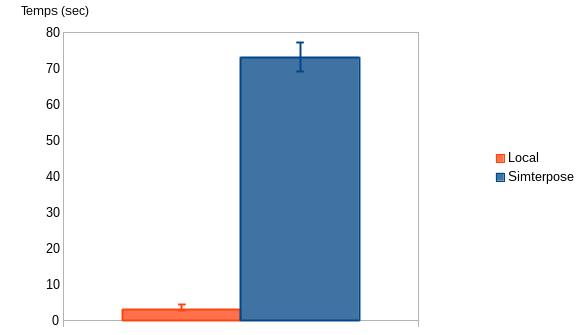
\includegraphics[scale=0.5]{mesures/graph/Littlemsg_local.jpg}
    \caption{Temps d'exécution lors de l'envoi d'un million de messages de 128o avec et sans Simterpose.}
    \label{Network_Little_Local}
\end{figure}

Dans le cas de l'envoi de plusieurs petits messages le temps moyen d'exécution en local est d'environ 3 secondes, avec Simterpose il est de 72 secondes en \textit{full mediation} et de 75 secondes en \textit{address translation}.

Lors de l'envoi d'un gros message le temps d'exécution moyen est de 0,01 secondes pour exécuter l'application en local alors qu'avec Simterpose il oscille entre 1 et 1,1 secondes selon le type de médiation.

\paragraph{Quelle médiation pour quel type d'application}
 Cette seconde expérience vise à comparer les deux médiations que nous avons implémentées. Pour cela, en suivant le protocole présenté plus haut on va exécuter les deux applications réseau choisi en utilisant les deux types de médiations. Les résultats de notre expérience sont présentés Figures \ref{Network_Big_Mediation} et \ref{Network_Little_Mediation}.

 \begin{figure}[H]
  \centering
    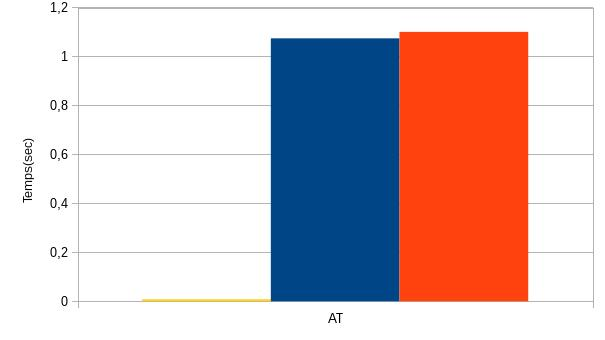
\includegraphics[scale=0.5]{mesures/graph/Bigmsg.jpg}
    \caption{Temps d'exécution lors de l'envoi d'un message de 1Mo en \textit{full mediation} et \textit{address translation}.}
    \label{Network_Big_Mediation}
\end{figure}

\begin{figure}[H]
  \centering
    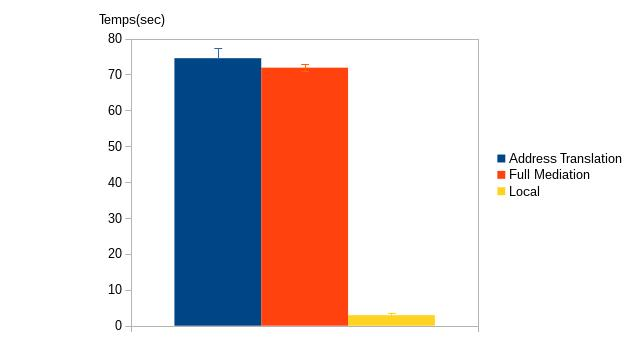
\includegraphics[scale=0.5]{mesures/graph/Littlemsg.jpg}
    \caption{Temps d'exécution lors de l'envoi d'un million de messages de 128o en \textit{full mediation} et \textit{address translation} avec et sans Simterpose.}
    \label{Network_Little_Mediation}
\end{figure}

Lors de l'envoi de nombreux petits messages, on peut constater que la \textit{full mediation} est plus rapide que l'\textit{address translation} avec un écart moyen de 3\%.

Lorsque l'on envoie un gros message, on constate que l'écart moyen entre les deux types de médiation est de 2.5\%.

\subsubsection{Analyse}
\paragraph{Overhead concernant le temps d'exécution}
Si l'on souhaite réellement mettre en place notre émulateur, dans le cas de l'envoi de plusieurs petits messages, l'exécution prendra 25 fois plus de temps et lors de l'envoi d'un gros message, elle prendra 100 fois plus de temps. Cet écart s'explique par les nombreux appels systèmes et changements de contexte que nécessite Simterpose de par son utilisation coûteuse de \texttt{ptrace} en plus de l'exécution de l'appel système lui-même lorsqu'on utilise l'\textit{address translation}. Cette expérience constitue cependant le pire scénario possible, avec un très grand nombre de petits messages échangés dans l'application.

\paragraph{Quelle médiation pour quel type d'application}
Lorqu'on utilise l'\textit{address translation} l'envoi de messages génère des appels systèmes et changements de contexte qui n'ont pas lieu en \textit{full mediation} puisque dans ce cas, comme nous l'avons expliqué en section \ref{paragraph:FULL_MEDIATION}, les appels systèmes ne sont pas exécutés. Ces derniers étant coûteux cela explique pourquoi l'\textit{address translation} est moins rapide. De plus, en \textit{full mediation}, même si les appels systèmes sont bloqués, nous utilisons l'appel système \texttt{ptrace} pour effectuer nous-même les appels demandés par l'application que nous avons bloqués. Cette méthode même si elle reste moins coûteuse que l'exécution de l'appel système demandé consomme des cycles CPU, ce qui explique le faible écart entre les temps d'exécution moyen des deux types de médiation.

Nous pensons que lors de l'envoi d'un gros message l'\textit{address translation} est légèrement plus rapide car nous envoyons un seul message de 1Mo de données. En effet, même si en \textit{full mediation} on a beaucoup moins de changement de contexte de par le blocage des appels systèmes ici on ne fait qu'un seul appel et la faible différence entre les deux médiations ne peut donc être dûe à cela. Par contre, lors de l'envoi d'un tel message il faut prendre en compte la gestion de la mémoire car le message doit être stocké avant de pouvoir être envoyé par morceau sur le réseau. Ainsi, si on ne gère pas la mémoire de façon efficace on surconsomme des cycles CPU lorsqu'on accède à cette dernière. Or, nous n'avons pas encore mis en place de politique de gestion de mémoire particulière pour Simterpose. Néanmoins, les résultats ont une plus grande variabilité des temps d'exécution en \textit{address translation} qu'en \textit{full mediation}. On peut donc supposer qu'avec une politique de gestion mémoire aussi efficace que celle qui est utilisée par le système la \textit{full mediation} serait probablement plus rapide que l'\textit{address translation} comme dans l'expérience précédente.

 Ainsi, lors de l'envoi de nombreux messages il vaut mieux privilégier la \textit{full mediation}. De plus, les deux médiations se valent lorsqu'on souhaite envoyer de gros messages.
\subsubsection{Conclusion}

Pour notre première expérience, le surcoût mesuré est certes important, mais indique que notre approche reste utilisable même dans ce cas.

De plus, pour notre seconde expérience la faible durée d'exécution d'une expérience nous permet de considérer que l'\textit{overhead} dû à la mise en place de Simterpose est acceptable.

Ainsi, nous pouvons conclure que ce type de virtualisation est possible pour le réseau.

\subsection{Temps}
\label{section:temps}

Dans la section \ref{subsubsection:time}, nous avons pu voir qu'il est important de gérer le temps que l'application voit s'écouler. En section \ref{section:work:time}, nous avons présenté l'implémentation qui a été choisie pour résoudre cette problématique. Maintenant, nous souhaitons évaluer ses performances.

\subsubsection{Protocole}
Pour évaluer notre implémentation nous n'allons pas utiliser les mêmes expériences que pour le réseau de communications car le but ici est d'intercepter les fonctions temporelles.

L'objectif principal étant de montrer qu'il est possible de faire de la virtualisation légère, nous souhaitons mesurer le surcoût ajouté par cette interception lors de l'exécution de Simterpose. Si ce surcoût est acceptable, on pourra considérer qu'il est également possible de mettre en place une virtualisation légère qui gère cette fonctionnalité. Nos expériences vont donc consister à comparer les temps d'exécution d'une application utilisant Simterpose avec et sans interception via \texttt{LD\_PRELOAD} pour chaque type de médiation. Néanmoins, nous pensons que le changement de médiation ne devrait pas influer sur les performances car chaque médiation intervient uniquement lorsqu'on souhaite effectuer des appels systèmes réseaux que l'on fasse de l'interception avec \texttt{LD\_PRELOAD} ou pas.

L'application qui a été créée pour effectuer nos expériences exécute différents appels à des fonctions temporelles (\texttt{ftime}, \texttt{time}, \texttt{gettimeofday}, \texttt{localtime}, \texttt{mktime}...). Le protocole utilisé pour exécuter l'application est le même que celui utilisé pour tester le réseau de communications de Simterpose.

\subsubsection{Full mediation}
 Tout d'abord nous allons exécuter l'application qui effectue les appels temporels avec Simterpose en \textit{full mediation} sans \texttt{LD\_PRELOAD} et avec \texttt{LD\_PRELOAD}. Les résultats de l'expérience sont présentés Figure \ref{Temps_FM}. On constate que le temps d'exécution avec interception via \texttt{LD\_PRELOAD} est plus ou moins constant (environ 1,03 secondes), alors que celui sans interception varie énormément, entre 0,82 et 1,13 secondes. Cela est dû au fait que lorsqu'on appelle des fonctions temporelles sans interception via \texttt{LD\_PRELOAD} la bibliothèque \texttt{VDSO} est appelée pour gérer l'appel et accéde elle-même à la mémoire. Cet accès n'a pas un coût constant puisqu'il dépend de la charge du système qui varie en permanence même si on ne fait tourner que notre application et aucune autre en parallèle. Ainsi, le temps d'exécution peut varier comme c'est la cas ici alors qu'il est stable quand on utilise \texttt{LD\_PRELOAD} puisqu'on empèche ces accès. Néanmoins, en moyenne les deux expériences ont environ le même temps d'exécution, 1 seconde pour la première et 1,02 secondes pour la deuxième. On peut donc considérer que l'interception via \texttt{LD\_PRELOAD} a un surcoût négligeable lorsqu'on utilise Simterpose en \textit{full mediation}.

\begin{figure}[H]
  \centering
    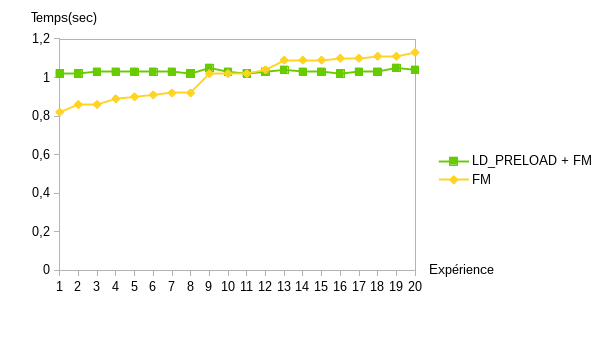
\includegraphics[scale=0.80]{mesures/graph/Temps_FM.png}
    \caption[Temps d'exécution d'une application temporelle en \textit{full mediation}] {Temps d'exécution d'une application temporelle en \textit{full mediation} avec interception via \texttt{LD\_PRELOAD} et sans interception.}
    \label{Temps_FM}
\end{figure}

\subsubsection{Address translation}
Nous allons maintenant voir s'il en est de même  lorsqu'on exécute l'application qui effectue les appels temporels avec Simterpose en \textit{address translation} avec et sans intercpetion via \texttt{LD\_PRELOAD}. Les résultats cette expérience sont présentés Figure \ref{Temps_AT}. On constate ici aussi que le temps d'exécution avec interception via \texttt{LD\_PRELOAD} est plus ou moins constant (environ 1,02 seconde), alors que celui sans interception varie beaucoup, entre 0,86 et 1,12 secondes. Cela est dû comme précédement à l'utilisation de la bibliothèque \texttt{VDSO} en l'absence d'interception via \texttt{LD\_PRELOAD}. De plus, le temps d'exécution moyen des deux expériences est le même: 1,02 secondes. Dans ce cas, on peut dire que l'interceprtion via \texttt{LD\_PRELOAD} en \textit{address translation} n'a aucun surcoût.

\begin{figure}[H]
  \centering
    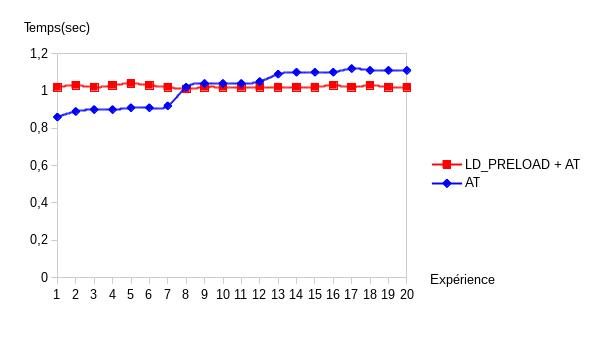
\includegraphics[scale=0.65]{mesures/graph/Temps_AT.jpg}
    \caption[Temps d'exécution d'une application temporelle en \textit{address translation}]{Temps d'exécution d'une application temporelle en \textit{address translation} avec interception via \texttt{LD\_PRELOAD} et sans interception.}
    \label{Temps_AT}
\end{figure}


Ainsi, nous avons pu voir que le surcoût dû à l'interception des fonctions temporelles via \texttt{LD\_PRELOAD} est inexistant en \textit{address translation} et qu'il est négligeable \textit{full mediation} (environ 2\%). On peut donc considérer que nous avons réussi à mettre en place une virtualisation légère qui gère également l'écoulement du temps et qui plus est de façon particulièrement efficace. De plus, en comparant les deux graphiques présentés Figure \ref{Temps_FM} et \ref{Temps_AT}, on voit bien que les courbes d'interception via \texttt{LD\_PRELOAD} se superposent et qu'il en est de même pour celles sans interception quelque soit la médiation utilisée. Le changement de médiation n'influe donc par sur les performances d'interception avec \texttt{LD\_PRELOAD}. Cela confirme l'hypothèse que nous avions fait.

\vspace{0.5cm}

Dans cette section nous avons analysé les performances des fonctionnalités implémentées durant ce stage. Cela nous a permis de constater que malgré l'existence d'un sur-coût au niveau du temps d'exécution, il est parfaitement possible de mettre en place une virtualisation légère utilisant le réseau de communications et la gestion du temps que nous avons mis en place dans Simterpose. Le tableau suivant résume les différents \textit{overhead} de Simterpose.

\begin{table}[H]
\centering
\resizebox{\textwidth}{!}{%
\begin{tabular}{c|c|c|c|c|c|}
\cline{2-6}
                              & \multicolumn{2}{c|}{Réseau de communciations} & \multicolumn{2}{c|}{Débit}        & \multirow{2}{*}{Temps} \\ \cline{2-5}
                              & Grosses données       & Petites données       & Grosses données & Petites données &                        \\ \hline
\multicolumn{1}{|c|}{Minimal} & 0.9s                  & 64s                   & 1.1Mo/s         & 2o/s            & 0s                     \\ \hline
\multicolumn{1}{|c|}{Maximal} & 1.18s                 & 74.5s                 & 850ko/s         & 1.7o/s          & 0.23s                  \\ \hline
\multicolumn{1}{|c|}{Moyen}   & 1.1s                  & 70.1s                 & 909ko/s         & 1.8o/s          & 0.02s                  \\ \hline
\end{tabular}
}
\caption{\textit{Overhead} du temps d'exécution d'applications avec Simterpose et débit des échanges}
\label{global_overhead}
\end{table}


\newpage
\section{Travaux futurs}
\label{section:future_work}

Dans les deux sections précédentes nous avons pu voir le travail et les expériences qui ont été réalisés au cours de ce stage. Néanmoins, notre émulateur n'est pas encore complet et lors de la rédaction de ce rapport de nouvelles idées ont émergées mais n'ont pu être mises en place. Nous allons présenter ici les améliorations qui pourraient être apportées à Simterpose et les expériences possibles.


\subsection{Simterpose}
\subsubsection{Fonctionnalités manquantes de Simterpose}
Dans la section \ref{section:work}, nous avons présenté les deux fonctionnalités implémentées durant ce stage. Néanmoins, il reste encore deux fonctionnalités à gérer: les threads et le DNS.

L'implémentation pour la gestion des threads se fera par la double interception complémentaire de \texttt{ptrace} et \texttt{LD\_PRELOAD}, comme nous l'avions présenté dans la section \ref{section:threads}.

Pour gérer la résolution de nom avec le DNS, trois solutions avaient été proposées en section \ref{section:DNS}, résumées dans le tableau \ref{table:DNS}. La solution la plus intéressante semble être d'intercepter les fonctions liées à la résolution de noms.

\begin{table}[H]
  \centering
  \resizebox{\textwidth}{!}{%
    \begin{tabular}{c|c|c|c|ll}
      \cline{2-4}
      & {\bf \begin{tabular}[c]{@{}c@{}}Interception sur \\ le port 53\\ (DNS par défaut)\end{tabular}}                                                                                                 & {\bf \begin{tabular}[c]{@{}c@{}}Remplacer le fichier\\ \texttt{resolv.conf}\end{tabular}}                             & {\bf \begin{tabular}[c]{@{}c@{}}Interception des fonctions\\ liées à la \\ résolution de noms\end{tabular}} &  &  \\ \cline{1-4}
      \multicolumn{1}{|c|}{{\it \begin{tabular}[c]{@{}c@{}}Niveau\\ d'interception\end{tabular}}} & \begin{tabular}[c]{@{}c@{}}Appel\\ Système\end{tabular}                                                                                                                                         & X                                                                                                                       & Bibliothèque                                                                                                &  &  \\ \cline{1-4}
        \multicolumn{1}{|c|}{{\it \begin{tabular}[c]{@{}c@{}}Outils\\ disponibles\end{tabular}}}    & \texttt{ptrace}                                                                                                                                                                              & X                                                                                                                       & \texttt{LD\_PRELOAD}                                                                                      &  &  \\ \cline{1-4}
        \multicolumn{1}{|c|}{{\it Coût}}                                                            & Moyen                                                                                                                                                                                           & Faible                                                                                                                  & Faible                                                                                                      &  &  \\ \cline{1-4}
        \multicolumn{1}{|c|}{{\it \begin{tabular}[c]{@{}c@{}}Mise en\\ \oe uvre\end{tabular}}}      & Complèxe                                                                                                                                                                                        & Simple                                                                                                                  & Simple                                                                                                      &  &  \\ \cline{1-4}
        \multicolumn{1}{|c|}{{\it Problèmes}}                                                       & \begin{tabular}[c]{@{}l@{}}- Teste pour chaque\\  communication le port utilisé\\ - Redéfinition possible du\\ port utilisé par le protocole DNS\end{tabular} & \begin{tabular}[c]{@{}l@{}}- Charge de travail \\ sur l'utilisateur\\ (création du fichier)\end{tabular} & - Risque d'oubli de fonctions                                                          &  &  \\ \cline{1-4}
    \end{tabular}
  }
  \caption[Solutions proposées pour gérer la résolution de noms via le protocole DSN]{Solutions proposées pour gérer la résolution de noms via le protocole DSN dans Simterpose.}
  \label{table:DNS}
\end{table}

\subsubsection{Amélioration des fonctionnalités existantes de Simterpose}
En section \ref{subsubsection:fonctionnement_reseau}, nous avons présentés deux types de médiation qui ont été implémentées pendant ce stage: la \textit{full mediation} et l'\textit{address translation}. Comme nous l'avons vu en section \ref{section:work}, lorsque Simterpose utilise la \textit{full mediation} il utilise \texttt{ptrace} pour accéder aux données à envoyer et/ou recevoir.

Nous avons envisagé une autre solution appelée ``accès direct'' qui serait peut-être moins coûteuse que l'exécution de cet appel système pour ce type de requête. Ce troisième type de médiation consisterait à ouvrir l'espace d'adressage des deux processus qui sont en train de communiquer via Simterpose, accessible depuis \texttt{/proc/PID/mem}. On pourrait ainsi lire et écrire directement dans la mémoire du processus concerné. Il existe pour cela des appels systèmes qui permettent à l'hyperviseur d'optimiser les communications entre VM\footnote{\url{http://knem.gforge.inria.fr/}}. Nous pourrions utiliser ce mécanisme pour faire communiquer nos processus. Il serait intéressant de comparer l'efficacité de cette approche à celles déjà implémentées.

\subsection{Expériences}
Dans la section \ref{section:evaluation}, nous avons présenté les différents tests que nous avons réalisés. Pour nos expériences, nous avons utilisé des tailles de message fixe. Il pourrait être intéressant de faire des tests en tirant aléatoirement la taille des messages entre X octets Y Méga-octets. De plus, pour terminer ce stage, nous souhaitions faire exécuter à Simterpose une application de torrent, telle que BitTorrent, mais nous avons manqué de temps et cela reste à faire.

Le nombre de processus en cours d'exécution influant forcément sur les performances, on pourrait exécuter plusieurs processus espions en parallèle afin de voir comment évoluent les performances de Simterpose. Ainsi, nous pourrions savoir  combien de processus espions peuvent être lancés simultanément et donc évaluer la scalabilité de notre émulateur. Dans ce cas, il serait intéressant de mesurer l'impact d'une telle exécution sur la mémoire en plus du temps d'exécution. Cela nous permettrait également d'évaluer encore plus finement les deux types de médiations implémentées. Par exemple, on pourrait voir si l'avantage de l'\textit{address translation} est accru ou décru quand des centaines de processus l'utilisent simultanément.

Enfin, une fois que nous aurons un émulateur complet, nous vérifierons qu'il est toujours possible de répondre à notre problématique de virtualisation légère. Puis, nous pourrons essayer d'améliorer son efficacité en fonctions des choix d'implémentations définitifs qui auront été faits.




\newpage
\section{Conclusion}
\label{section:ccl}

L'objectif de ce stage était de montrer qu'il est possible de faire de la
virtualisation légère afin de tester des applications distribuées large échelle
quelconques. Pour cela, nous avons commencé par expliquer le concept de
virtualisation légère et pouruqoi nous l'avions choisi. Puis nous avons présenté
les outils permettant sa mise en place ainsi que les projets qui actuellement
font de la virtualisation légère pour différents types d'applications. Les
projets existants ne permettant pas de résoudre les quatre problèmes engendrés
par cette virtualisation (gestion du temps, des threads, des communications
réseaux et le DNS) et donc de tester n'importe quel type d'applications
distribués, un nouveau projet a été lancé.

L'émulateur Simterpose dévelopé au LORIA permet d'exécuter et de tester des
applications distribuées réelles, sans disposer de leur code source, dans un
environnement virtuel. Il se base sur la plateforme de simulation SimGrid pour
mettre en place l'environnement d'exécution dans lequel l'application pensera
s'exécuter. Pour maintenir la virtualisation, les actions des applications sont
interceptées et modifiées pour ensuite être exécutées. On utilise SimGrid pour
calculer la réponse de l'environnement virtuel aux différentes actions. La
solution proposée intercepte les actions à deux niveaux différents: appels
systèmes et bibliothèques. Simterpose permet également d'injecter diverses
fautes dans la simulation pour avoir une virtualisation plus réaliste.

Au début du stage, Simterpose gèrait plus ou moins bien les threads, le réseau
de communications n'était implémenté qu'en parti et les deux autres
fonctionnalités (temps et DNS) étaient inexistantes. Nous avons donc terminé
l'implémentation du réseau de communications et avons mis en place la gestion du
temps. Ces deux fonctionnalités ont nécessitées la création de nouveaux outils
et des améliorations ont été apportées à Simterpose. Cependant, comme nous avons
pu le voir notre émulateur n'est pas encore terminé. Néanmoins, nos expériences
nous ont permis de montrer qu'il est déjà possible de mettre en place une
virtualisation légère par interception pour tester des applications distribuées
quelconques pour les deux fonctionnalités que nous avons implémentées.


\newpage
\begin{appendices}
\chapter{Utilisation de Simterpose}

Pour utiliser Simterpose il faut lui fournir deux fichiers, un fichier de plateforme et un de déploiement, qui seront utilisés par SimGrid.

Le fichier de plateforme permet à SimGrid de mettre en place le réseau simulé. Dans ce fichier on définit plusieurs choses. Tout d'abord, on définit les hôtes présents sur le réseau. Pour chaque hôte, on spécifie un identifiant, une puissance de calcul et éventuellement une adresse IP(v4). Si on ne fournit aucune adresse IP à un n\oe ud, une adresse IP arbitraire lui sera alloué au début de la simulation. Ensuite, on définit toutes les routes du réseau. Pour cela, il faut fournir à chacune une bande passante, une latence, ainsi que les noeuds reliés.

Le fichier de déploiement quand à lui permet de définir la répartition de l'application distribuée sur la plateforme. Pour chaque processus utilisé, on va définir le n\oe ud qui va l'héberger parmi ceux présent dans le fichier de plateforme. On fournit également le binaire de l'application à exécuter et si besoin les paramètres nécessaires pour lancer l'application. De plus, il faut fournir un temps que nous appelons ``temps de début'' qui est utilisé par SimGrid pour lancer l'application quand son temps simulé a atteint le ``temps de début''.
\vspace{0.5cm}

Pour lancer Simterpose il y a plusieurs commandes en fonction du type d'exécution désirée.

\lstdefinestyle{customc}{
  belowcaptionskip=1\baselineskip,
  breaklines=true,
  xleftmargin=\parindent,
  language=sh,
  showstringspaces=false,
  basicstyle=\footnotesize\ttfamily,
  keywordstyle=\bfseries\color{blue},
  commentstyle=\itshape\color{green!40!black},
  identifierstyle=\color{blue},
  stringstyle=\color{violet},
}
\lstset{escapechar=@,style=customc, caption={}}
\begin{lstlisting}
#Pour une exécution simple (avec interception réseau uniquement)
> sudo simterpose -s platform.xml deploiement.xml

#Pour une exécution avec en plus l'interception du temps
> sudo LD_PRELOAD=lib.so -s platform.xml deploiement.xml

#Pour utiliser un débogueur
> sudo simterpose ``gdb --args'' -s platform.xml deploiement.xml
#ou
> sudo simterpose valgrind -s platform.xml deploiement.xml
\end{lstlisting}
\end{appendices}


\newpage
% Bib
\bibliographystyle{plainnat}
\bibliography{src/10.Biblio} % The file containing the bibliography
\label{fin}

\end{document}
